%-----------------------------------------------------------------------------%
\chapter{\babTiga}
%-----------------------------------------------------------------------------%

%-----------------------------------------------------------------------------%
\section{Kedudukan dan Koordinasi}
%-----------------------------------------------------------------------------%
Selama masa kerja magang yang berlangsung dari 05 Januari 2026 hingga 20 Mei 2026, posisi yang dijalankan adalah \textit{Full-Stack Developer}. Dalam struktur operasional proyek pengembangan \textit{HR Safety Campus}, pelaksanaan magang berada di bawah pengawasan langsung supervisor atau pembimbing lapangan yang bertugas memberikan arahan teknis dan mengevaluasi progres mingguan.

Selain berkoordinasi dengan supervisor, interaksi juga dilakukan dengan klien dan tim operasional lapangan. Koordinasi ini sangat krusial, terutama ketika melakukan validasi temuan data pekerja yang ganda atau duplikat sebelum melakukan proses unggah (\textit{upload}) ke dalam basis data utama.

%-----------------------------------------------------------------------------%
\section{Tugas yang Dilakukan}
\label{sec:tugas}
%-----------------------------------------------------------------------------%
Sebagai \textit{Full-Stack Developer}, fokus utama pekerjaan ini adalah membangun aplikasi \textit{HR Safety Campus} dari sisi antarmuka (\textit{frontend}) hingga ke logika peladen (\textit{backend}) dan basis data. Berikut adalah rincian tugas yang telah dilakukan selama magang:

\begin{enumerate}
    \item \textbf{Penyiapan Lingkungan Pengembangan (\textit{Development Environment}):} Melakukan konfigurasi perangkat kerja pada laptop Asus Vivobook, termasuk instalasi \textit{Composer}, pengaturan ekstensi PHP, dan penyiapan struktur proyek berbasis Laravel.
    \item \textbf{Pengembangan Antarmuka Pengguna:} Merancang dan mengimplementasikan tampilan aplikasi web yang responsif untuk modul registrasi tenaga kerja, cetak \textit{permit}, dan klaim transportasi menggunakan \textit{Tailwind CSS} guna memastikan performa visual halaman manajemen data tetap optimal \cite{nandan2024tailwind}.
    \item \textbf{Pengembangan Logika \textit{Backend}:} Membangun fungsi-fungsi inti aplikasi menggunakan bahasa pemrograman PHP dengan kerangka kerja Laravel yang mengadopsi pola arsitektur \textit{Model-View-Controller} (MVC) \cite{rahmawati2024mvc} dan pengembangan \textit{REST API} \cite{ariyanto2024restapi}. Proses ini mencakup pembuatan sistem keamanan dengan arsitektur \textit{Role-Based Access Control} (RBAC) untuk membatasi hak akses menu pengguna lapangan dan mencegah manipulasi data \cite{mary2025rbac}.
    \item \textbf{Pengelolaan dan Migrasi Basis Data:} Melakukan transisi data dari sistem lama (Microsoft Access) ke MySQL. Tugas ini mencakup eksekusi perintah SQL seperti \textit{TRUNCATE} untuk pembersihan data awal, penanganan \textit{file} CSV, dan identifikasi serta sinkronisasi sekitar 4.000 rekaman data karyawan.
\end{enumerate}

Rincian pekerjaan yang dilakukan setiap minggu selama pelaksanaan kerja magang dapat dilihat pada Tabel \ref{tbl_uraian}.

\begin{longtable}{|c | p{0.72\textwidth}| }
	\caption{Detail Pekerjaan yang Dilakukan}
	\label{tbl_uraian} \\
	\hline
	\textbf{Minggu Ke-} & \textbf{Pekerjaan yang Dilakukan} \\
	\hline
	\endfirsthead
	\multicolumn{2}{c}{\textit{Lanjutan Tabel \ref{tbl_uraian}}} \\
	\hline
	\textbf{Minggu Ke-} & \textbf{Pekerjaan yang Dilakukan} \\
	\hline
	\endhead
	\hline
	\endfoot
	\hline
	\endlastfoot
	1 & Observasi alur kerja sistem lama berbasis Microsoft Access serta identifikasi kebutuhan sistem baru bersama tim IT. \\
	\hline
	2 & Penyiapan \textit{environment} pengembangan (Laravel, Composer, ekstensi PHP, MySQL) dan inisialisasi struktur proyek. \\
	\hline
	3 & Perancangan skema basis data dan relasi antar tabel (karyawan, kontraktor, klaim, tarif, dan pengguna). \\
	\hline
	4 & Pengembangan kerangka antarmuka dasar menggunakan \textit{Tailwind CSS} serta penyiapan tata letak (\textit{layout}) utama aplikasi. \\
	\hline
	5 & Implementasi fitur Registrasi Tenaga Kerja bagian formulir input data pribadi dan data kepegawaian. \\
	\hline
	6 & Integrasi data wilayah IndoRegion (provinsi, kabupaten/kota, kecamatan) berbasis pencarian bertingkat pada formulir registrasi. \\
	\hline
	7 & Pengembangan penomoran ID karyawan otomatis serta fitur cetak ID Card dalam format PDF menggunakan \textit{library} FPDF. \\
	\hline
	8 & Implementasi sistem autentikasi dan arsitektur \textit{Role-Based Access Control} (RBAC) pada \textit{backend}. \\
	\hline
	9 & Pengembangan fitur Manajemen Pengguna (\textit{User Management}) beserta pengaturan hak akses granular per menu. \\
	\hline
	10 & Pengembangan fitur Manajemen Tarif Transport (\textit{Manage Rates}) berikut mekanisme pengarsipan tarif lama. \\
	\hline
	11 & Pengembangan fitur Klaim Transport bagian \texttt{CLAIM\_IN} beserta aturan validasi minimal masa kerja. \\
	\hline
	12 & Pengembangan fitur Klaim Transport bagian \texttt{CLAIM\_OUT} dan perhitungan nominal klaim otomatis berbasis tarif. \\
	\hline
	13 & Pengembangan fitur Surat Izin Keluar (\textit{Exit Permits}) termasuk penomoran surat jalan otomatis. \\
	\hline
	14 & Implementasi pencetakan surat jalan dalam format A4 \textit{landscape} dan pembaruan status karyawan otomatis. \\
	\hline
	15 & Pengembangan fitur Persetujuan Karyawan (\textit{Employees Approval}) dengan evaluasi kelengkapan data otomatis. \\
	\hline
	16 & Pengujian fungsional menyeluruh terhadap keenam fitur utama serta perbaikan \textit{bug} yang ditemukan. \\
	\hline
	17 & Pembersihan data (\textit{data cleansing}) terhadap data tenaga kerja dari sistem lama dan normalisasi format data. \\
	\hline
	18 & Pengembangan skrip deteksi duplikasi NIK dan migrasi sekitar 4.000 rekaman data ke basis data MySQL. \\
	\hline
	19 & Penyusunan laporan data bermasalah untuk klien serta pemetaan kode kontraktor (\textit{contractor\_id}) dari data vendor. \\
	\hline
	20 & Evaluasi akhir, perapian kode, dan penyerahan dokumentasi proyek kepada pihak \textit{supervisor}. \\
\end{longtable}

%-----------------------------------------------------------------------------%
\section{Uraian Pelaksanaan Kerja Magang}
%-----------------------------------------------------------------------------%
Bagian ini menguraikan secara umum pelaksanaan pekerjaan selama kerja magang, mencakup proses perancangan dan pengembangan keenam fitur utama sistem \textit{HR Safety Campus}, kendala-kendala yang ditemukan selama pelaksanaan, serta solusi yang diterapkan untuk mengatasinya.

%-----------------------------------------------------------------------------%
\subsection{Perancangan Sistem}
%-----------------------------------------------------------------------------%
Sebelum masuk ke tahap implementasi, dilakukan perancangan struktur sistem \textit{HR Safety Campus} dalam bentuk \textit{site map} dan \textit{flowchart} untuk setiap fitur utama, guna memastikan alur navigasi dan logika bisnis terdefinisi dengan jelas sebelum proses pengkodean dimulai.

\subsubsection*{Site Map Sistem}

Struktur navigasi sistem \textit{HR Safety Campus} terdiri atas halaman Login yang mengarah ke Main Menu sebagai pusat navigasi, dengan delapan modul utama di bawahnya. Site map lengkap sistem ditunjukkan pada Gambar \ref{fig:sitemap}.

\begin{figure}[H]
\centering
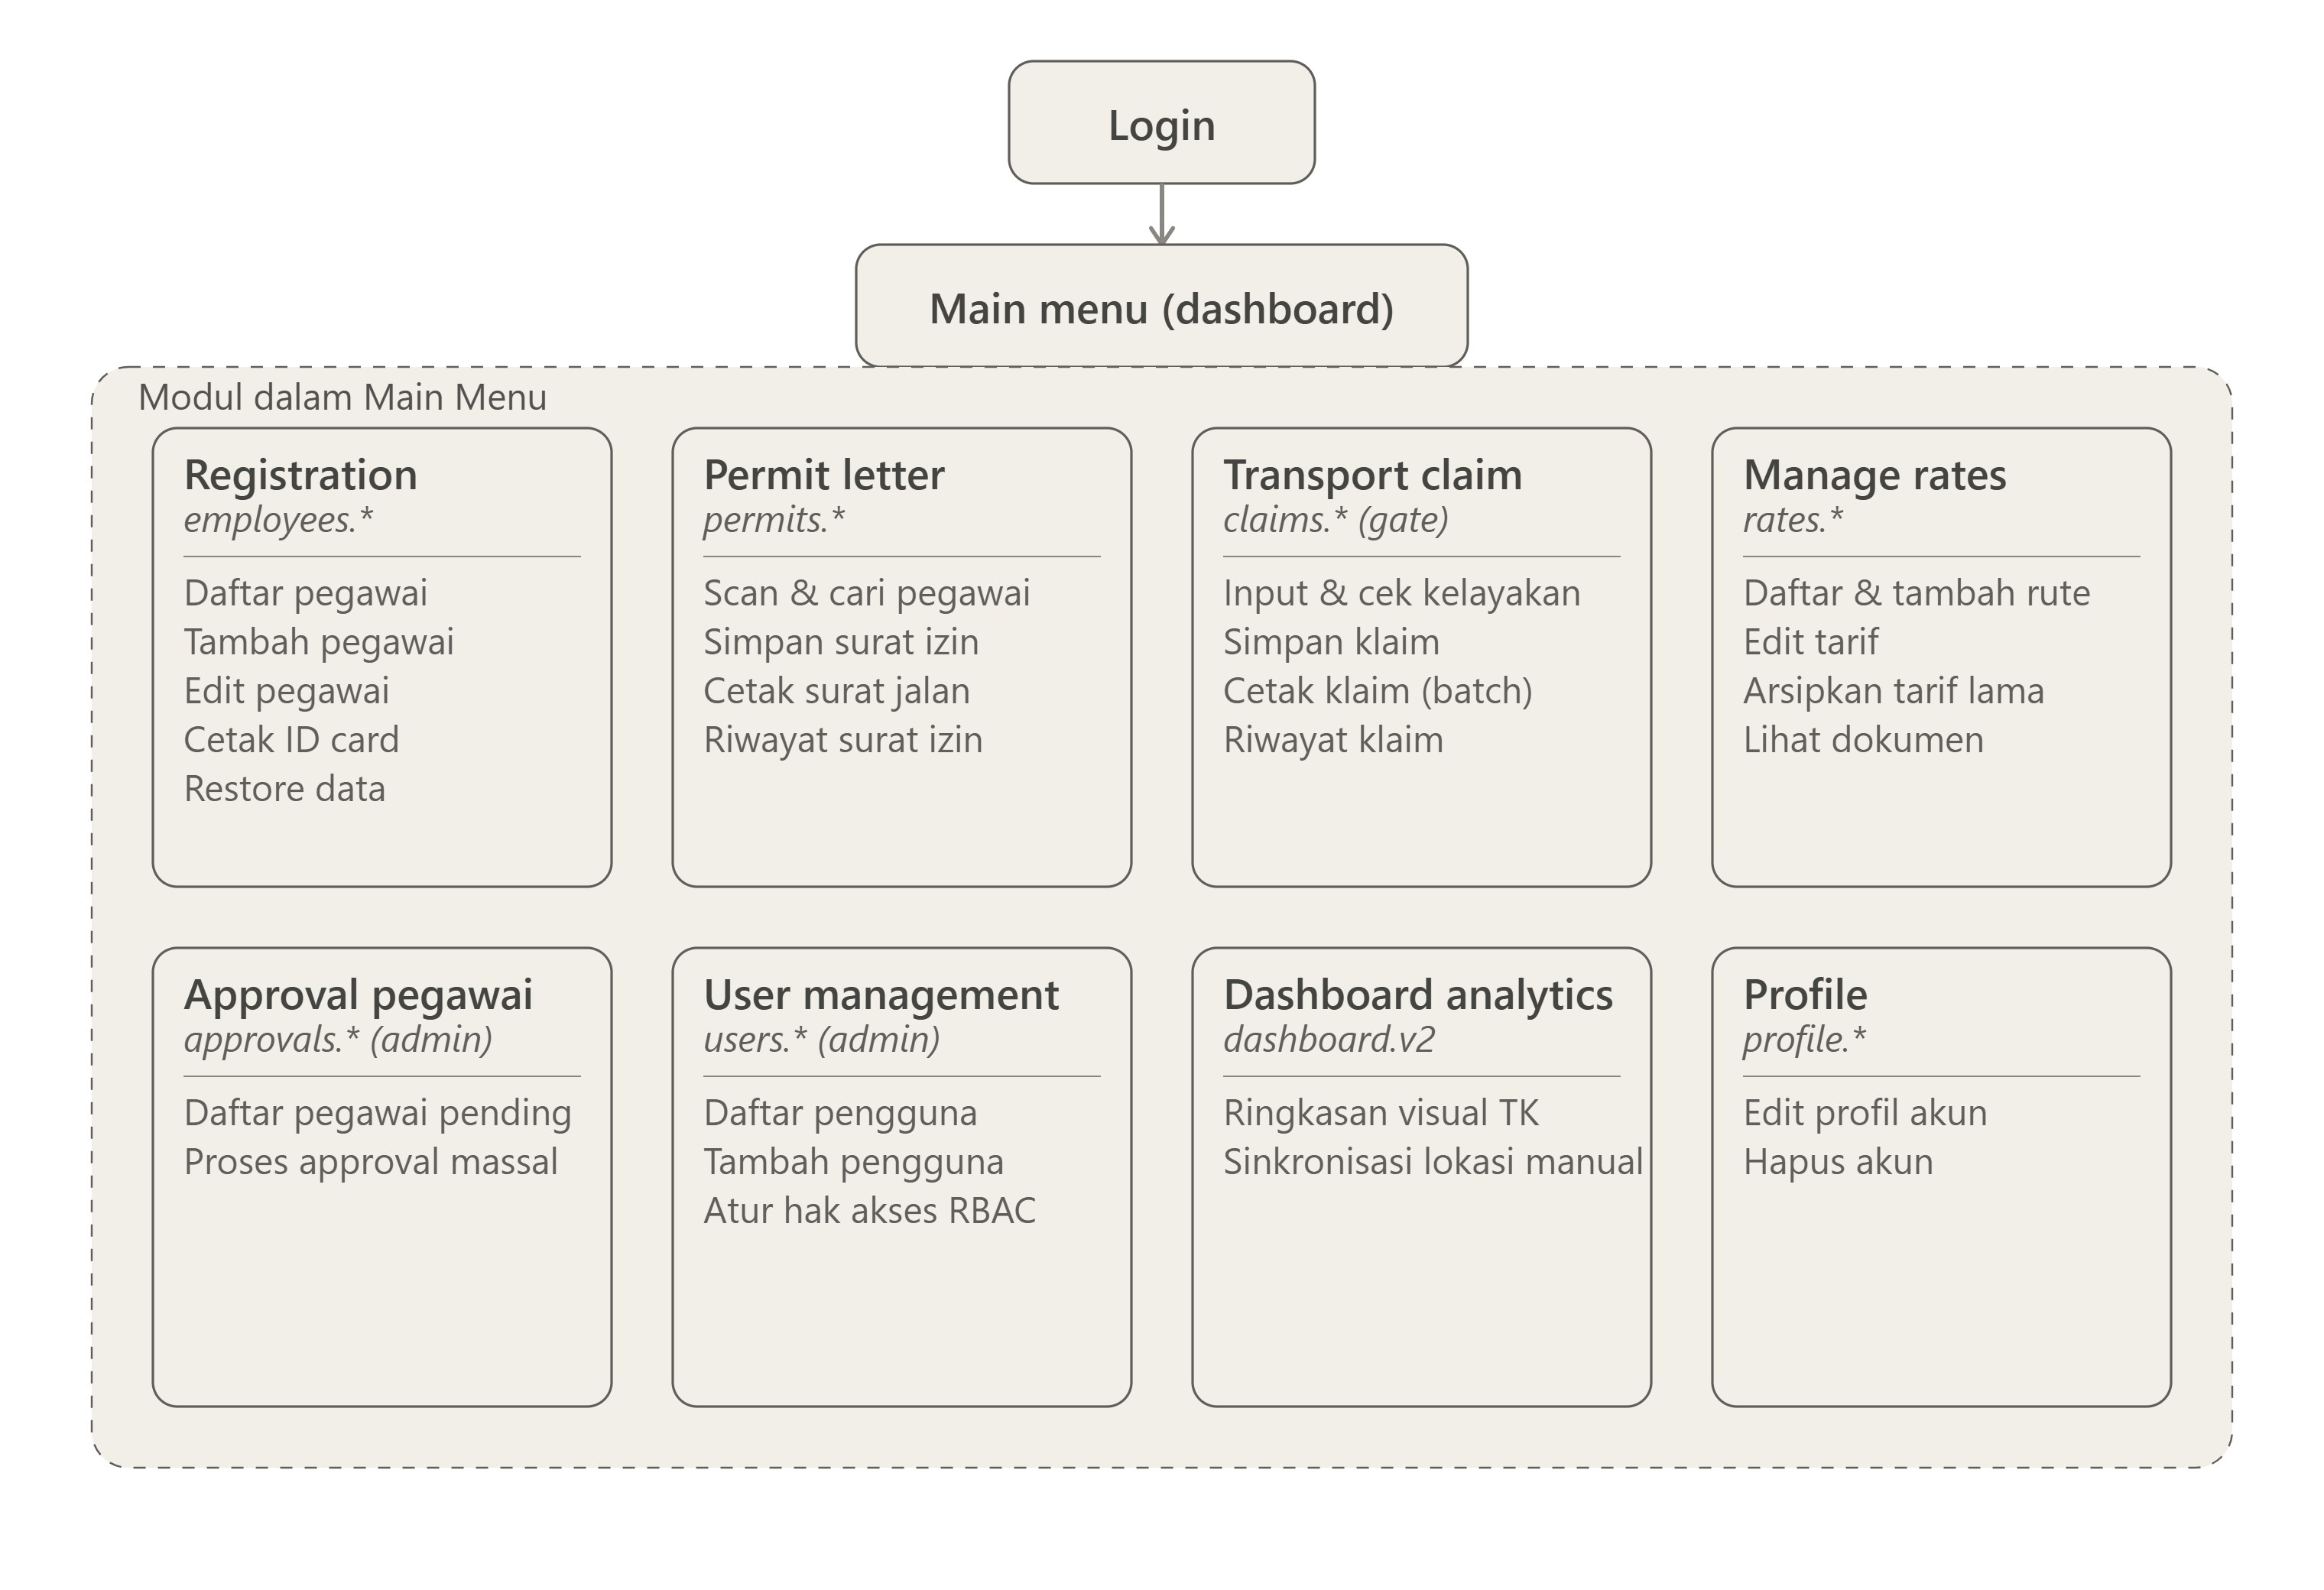
\includegraphics[width=0.95\textwidth]{assets/pics/sitemap.png}
\caption{Site map sistem HR Safety Campus}
\label{fig:sitemap}
\end{figure}

Gambar \ref{fig:sitemap} menunjukkan bahwa seluruh modul berada dalam satu Main Menu terpusat, dengan modul \textit{Transport Claim} dan grup \textit{Approval Pegawai}/\textit{User Management} dilindungi \textit{gate} akses khusus (\texttt{access-claim} dan \texttt{admin-only}) sebagaimana akan dijelaskan lebih lanjut pada bagian Manajemen Pengguna.

\subsubsection*{Flowchart Registrasi Tenaga Kerja}

Rancangan alur penomoran ID otomatis dan penentuan status karyawan sebagaimana diimplementasikan pada Kode \ref{lst:reg} ditunjukkan pada Gambar \ref{fig:flowchart-registrasi}.

\begin{figure}[H]
\centering
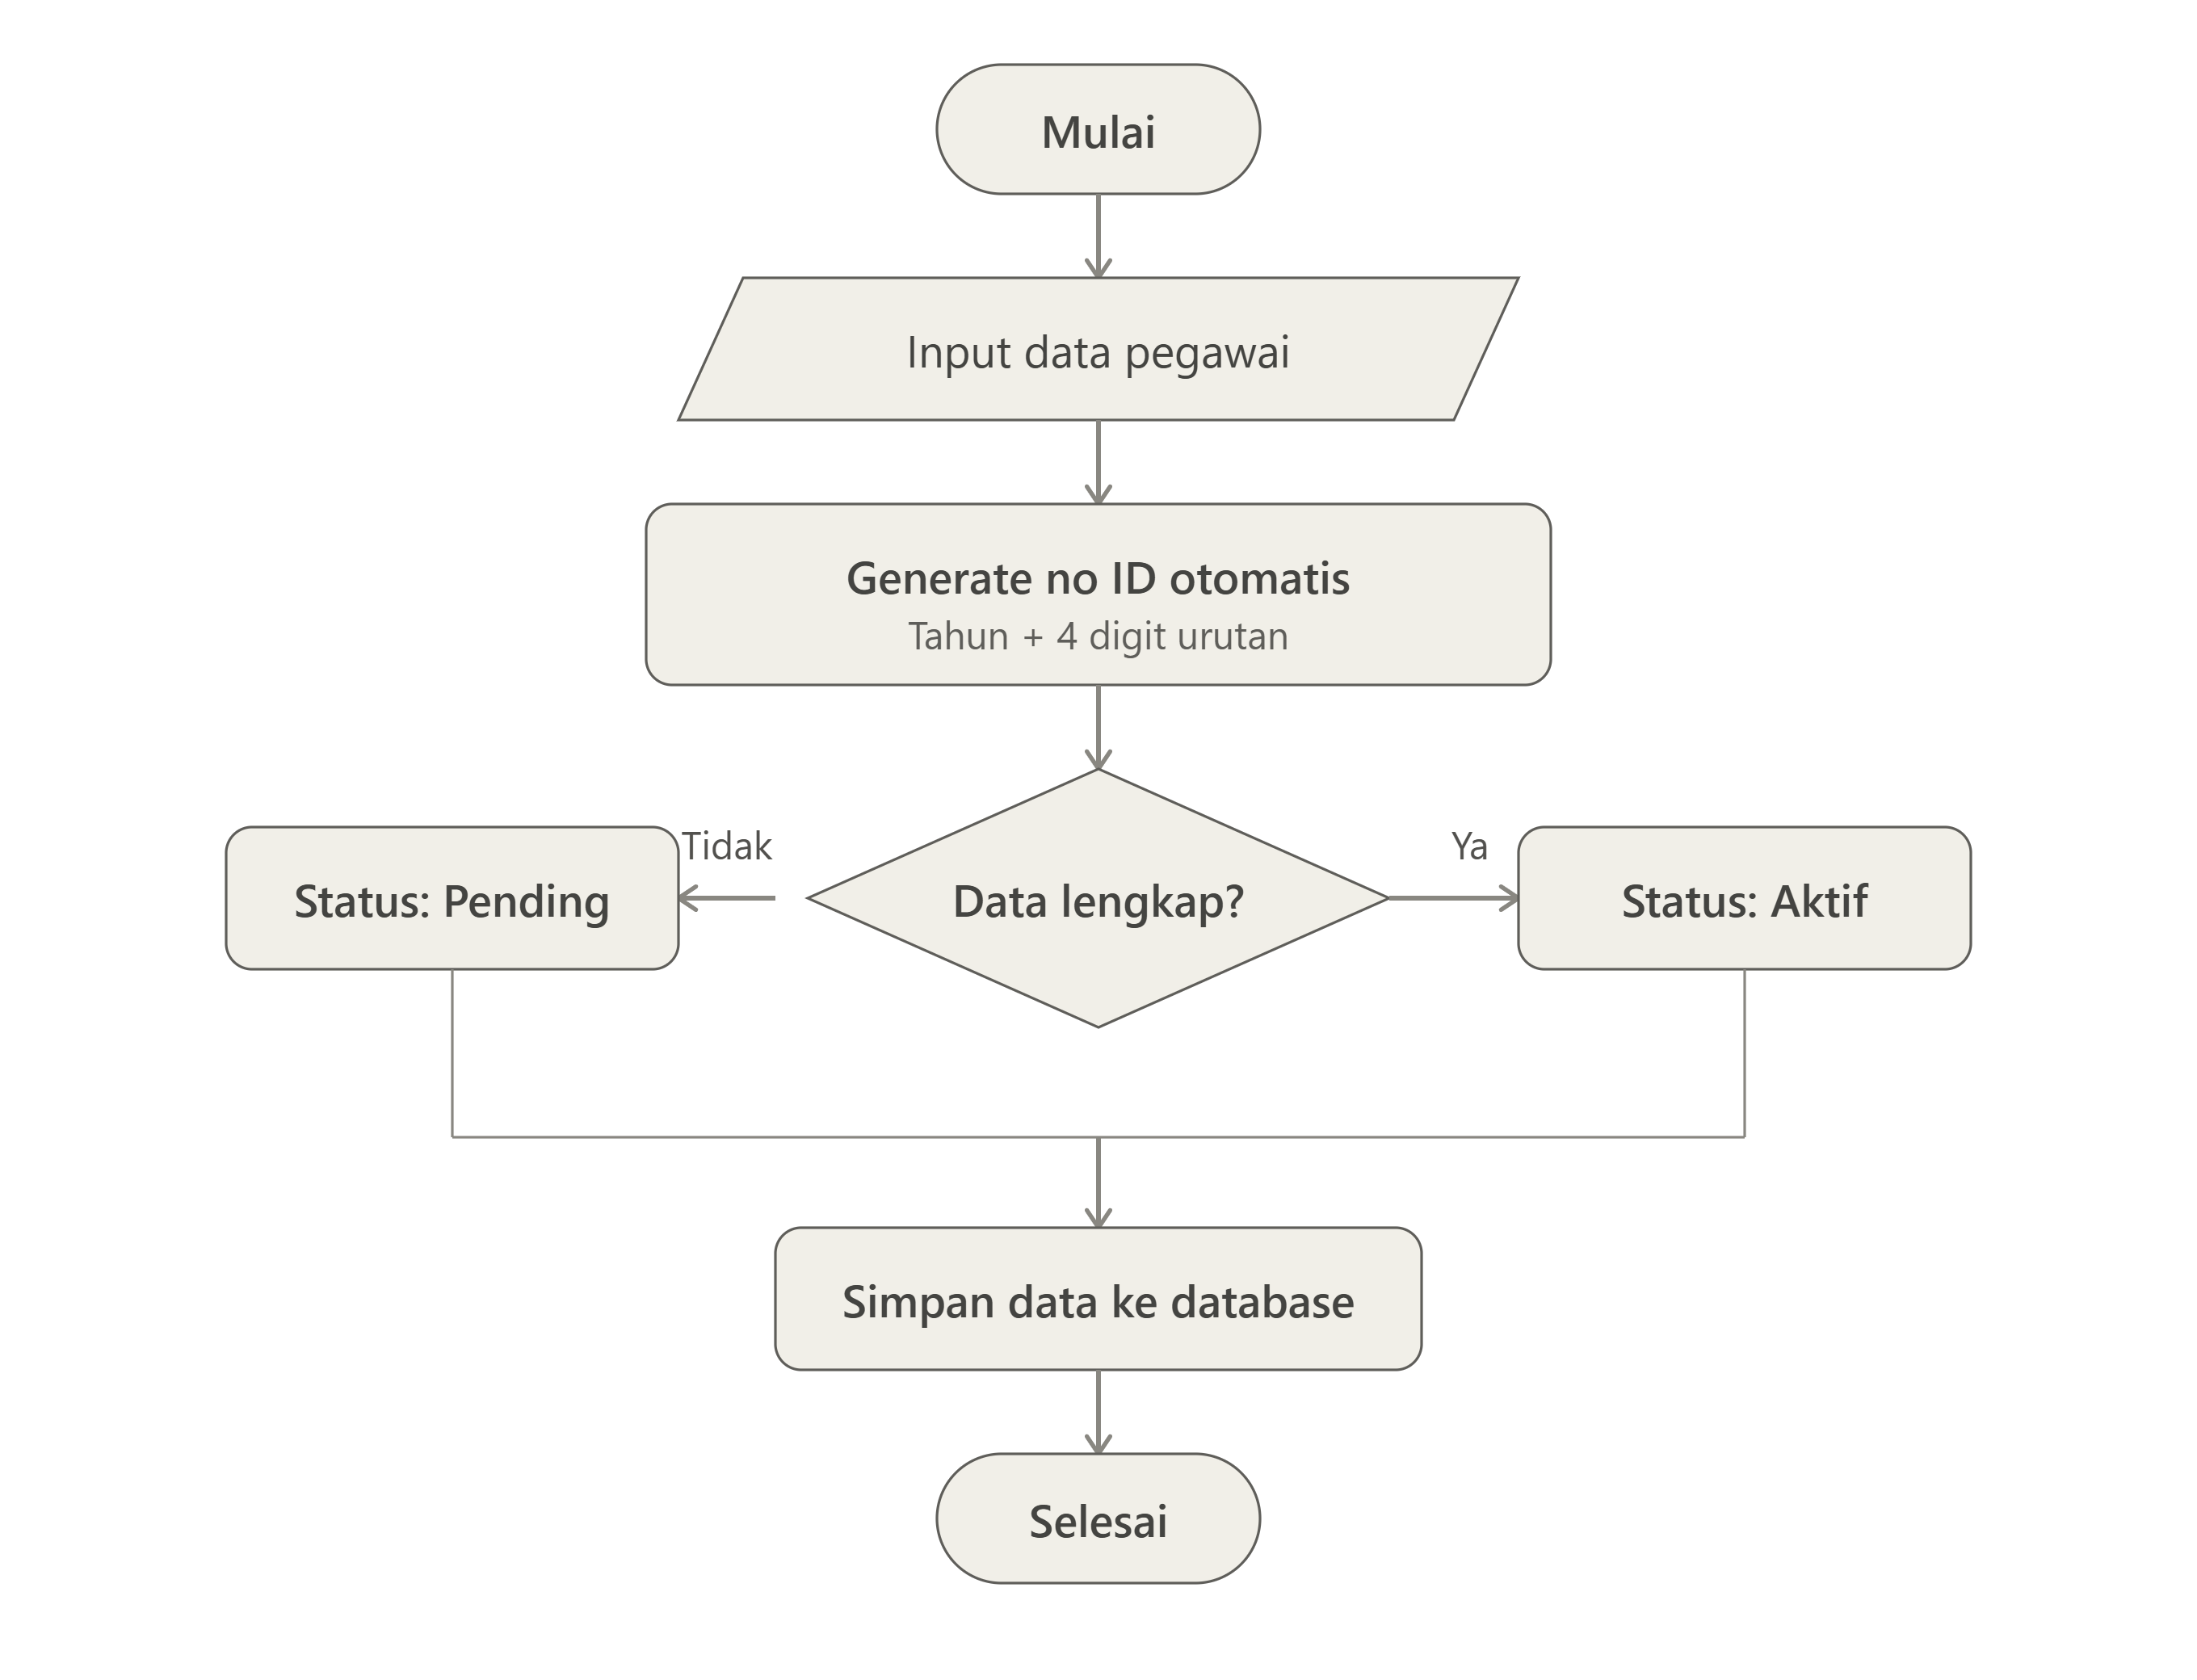
\includegraphics[width=0.8\textwidth]{assets/pics/flowchart_registrasi.png}
\caption{Flowchart proses Registrasi Tenaga Kerja}
\label{fig:flowchart-registrasi}
\end{figure}

\subsubsection*{Flowchart Klaim Transport}

Fitur Klaim Transport memiliki dua alur validasi terpisah, yaitu \texttt{CLAIM\_IN} (klaim kedatangan) dan \texttt{CLAIM\_OUT} (klaim kepulangan), masing-masing dengan aturan bisnis berlapis sebagaimana diimplementasikan pada Kode \ref{lst:claim}. Rancangan alur validasi \texttt{CLAIM\_IN} ditunjukkan pada Gambar \ref{fig:flowchart-claimin}.

\begin{figure}[H]
\centering
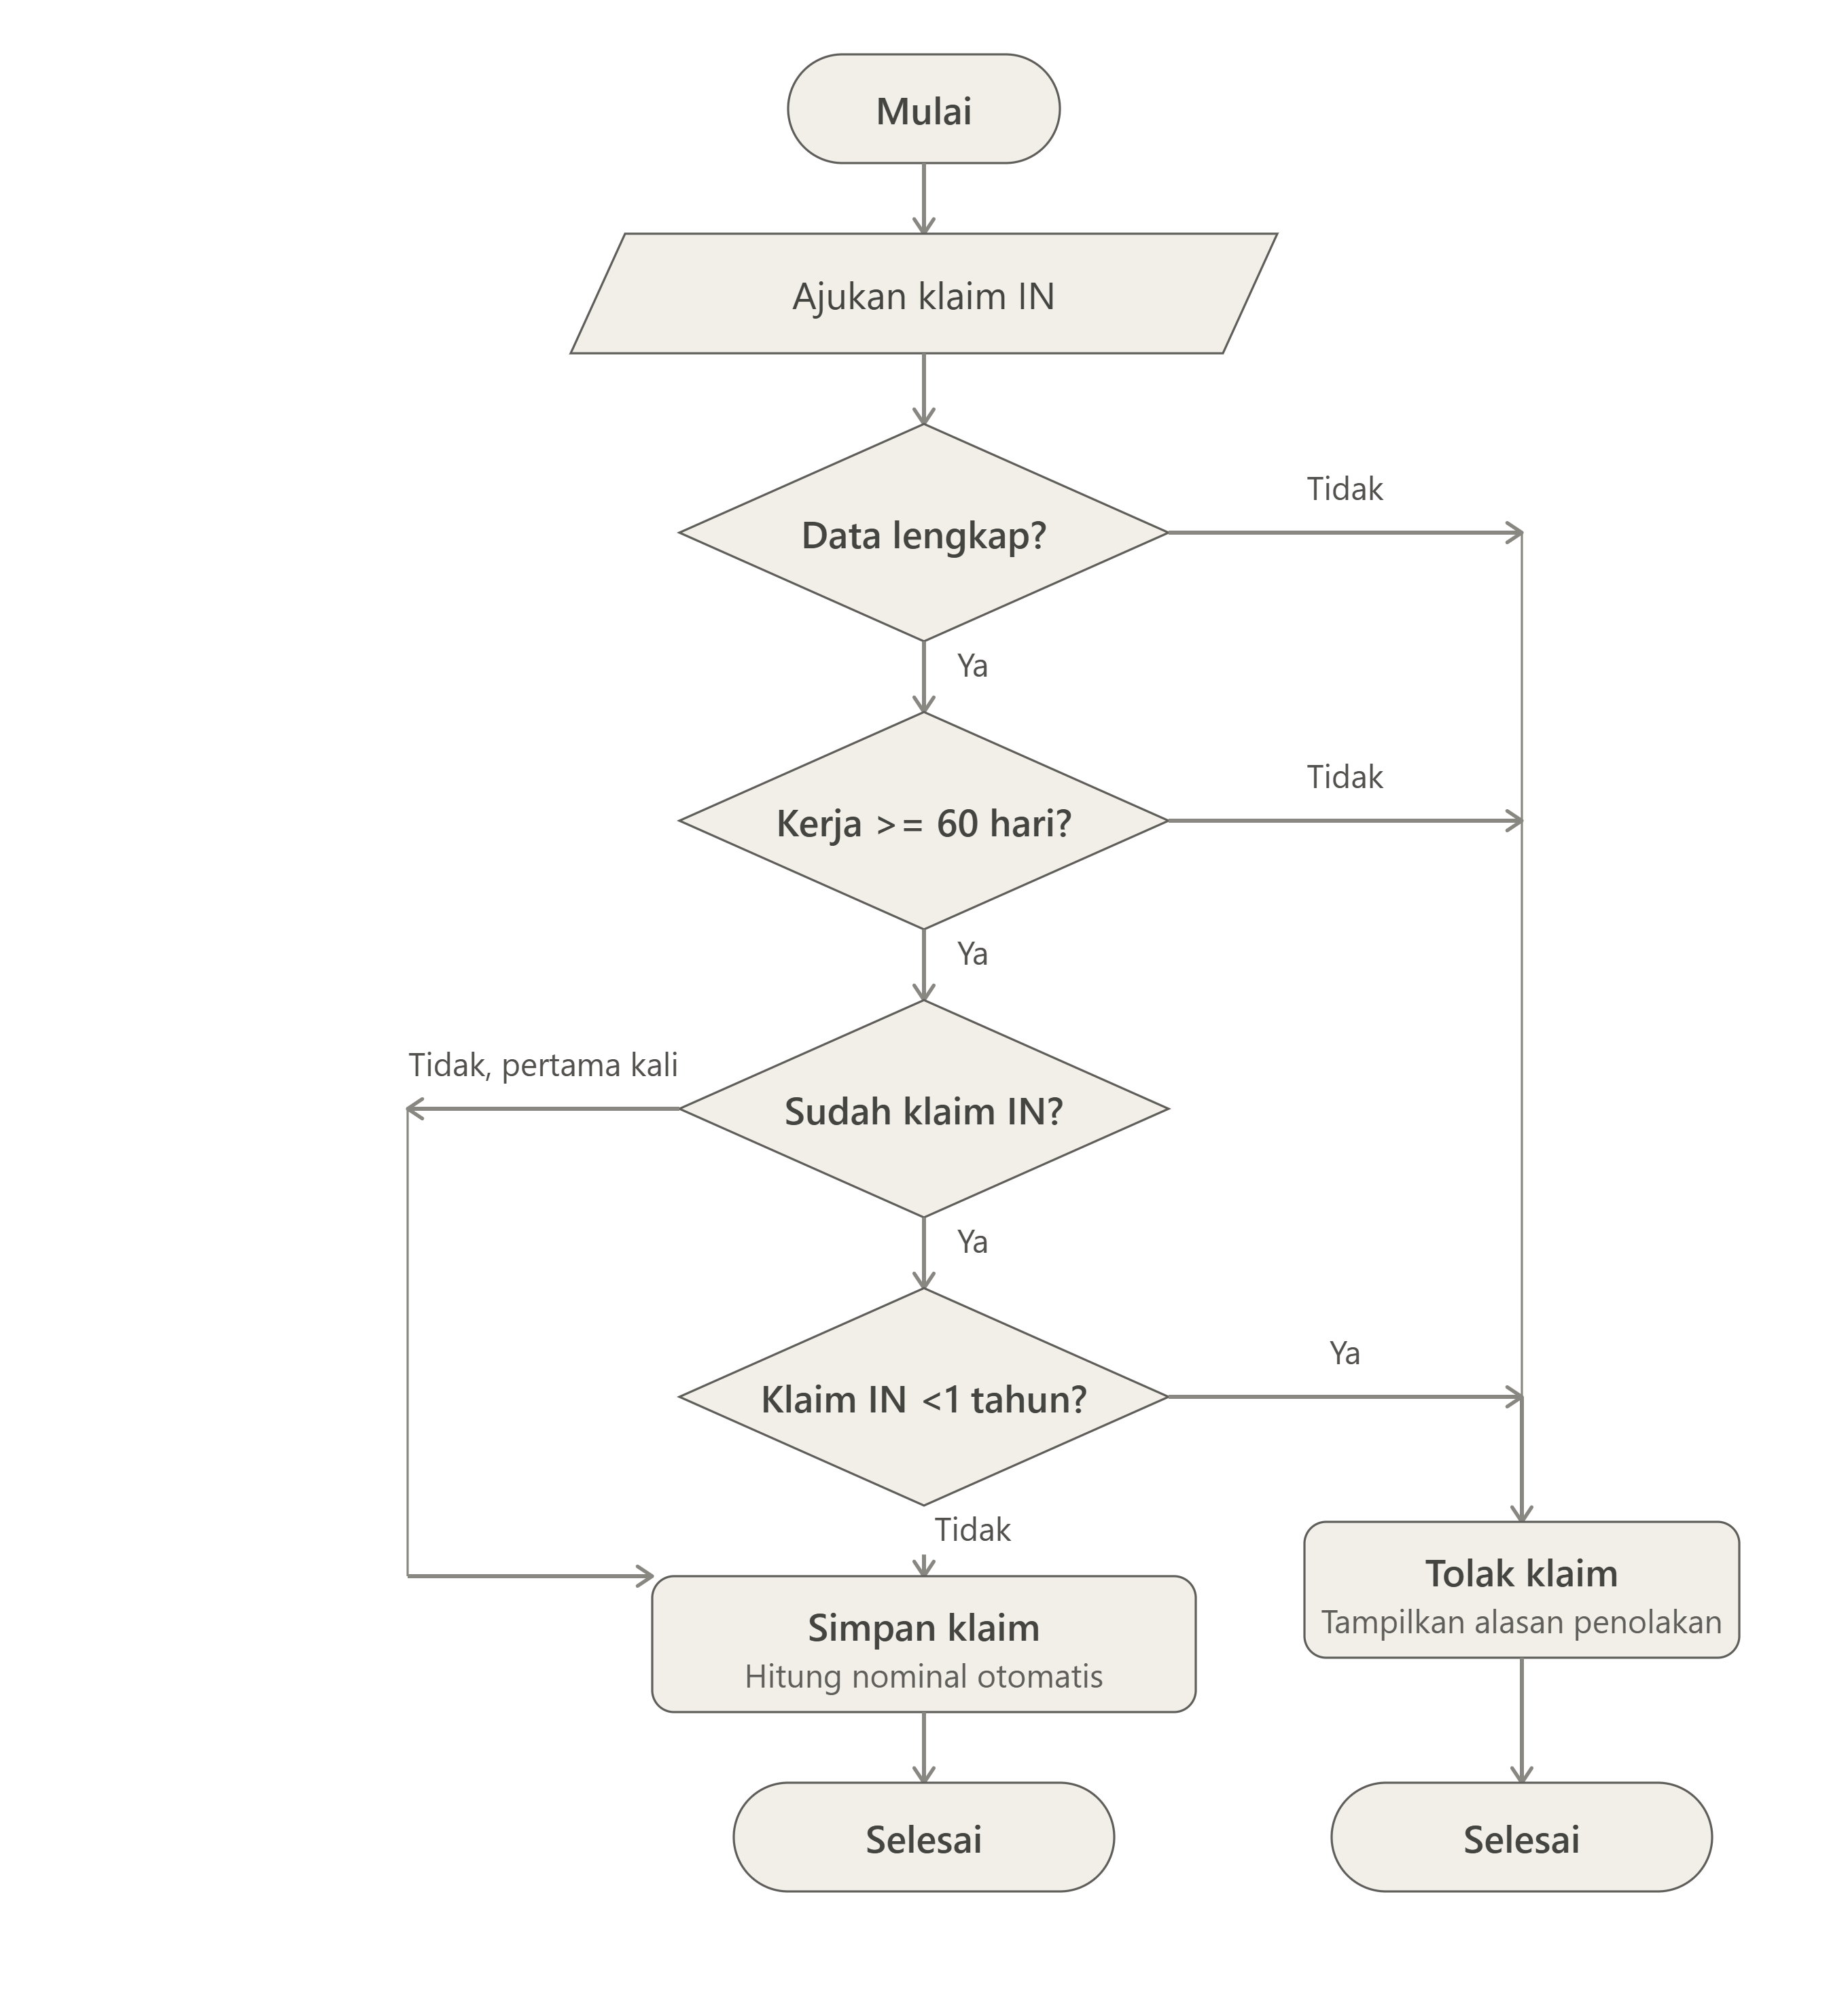
\includegraphics[width=0.85\textwidth]{assets/pics/flowchart_claim_in.png}
\caption{Flowchart validasi pengajuan Klaim Transport (CLAIM\_IN)}
\label{fig:flowchart-claimin}
\end{figure}

Sementara itu, rancangan alur validasi \texttt{CLAIM\_OUT} yang mencakup pengecualian khusus untuk departemen \textit{Plantation} ditunjukkan pada Gambar \ref{fig:flowchart-claimout}.

\begin{figure}[H]
\centering
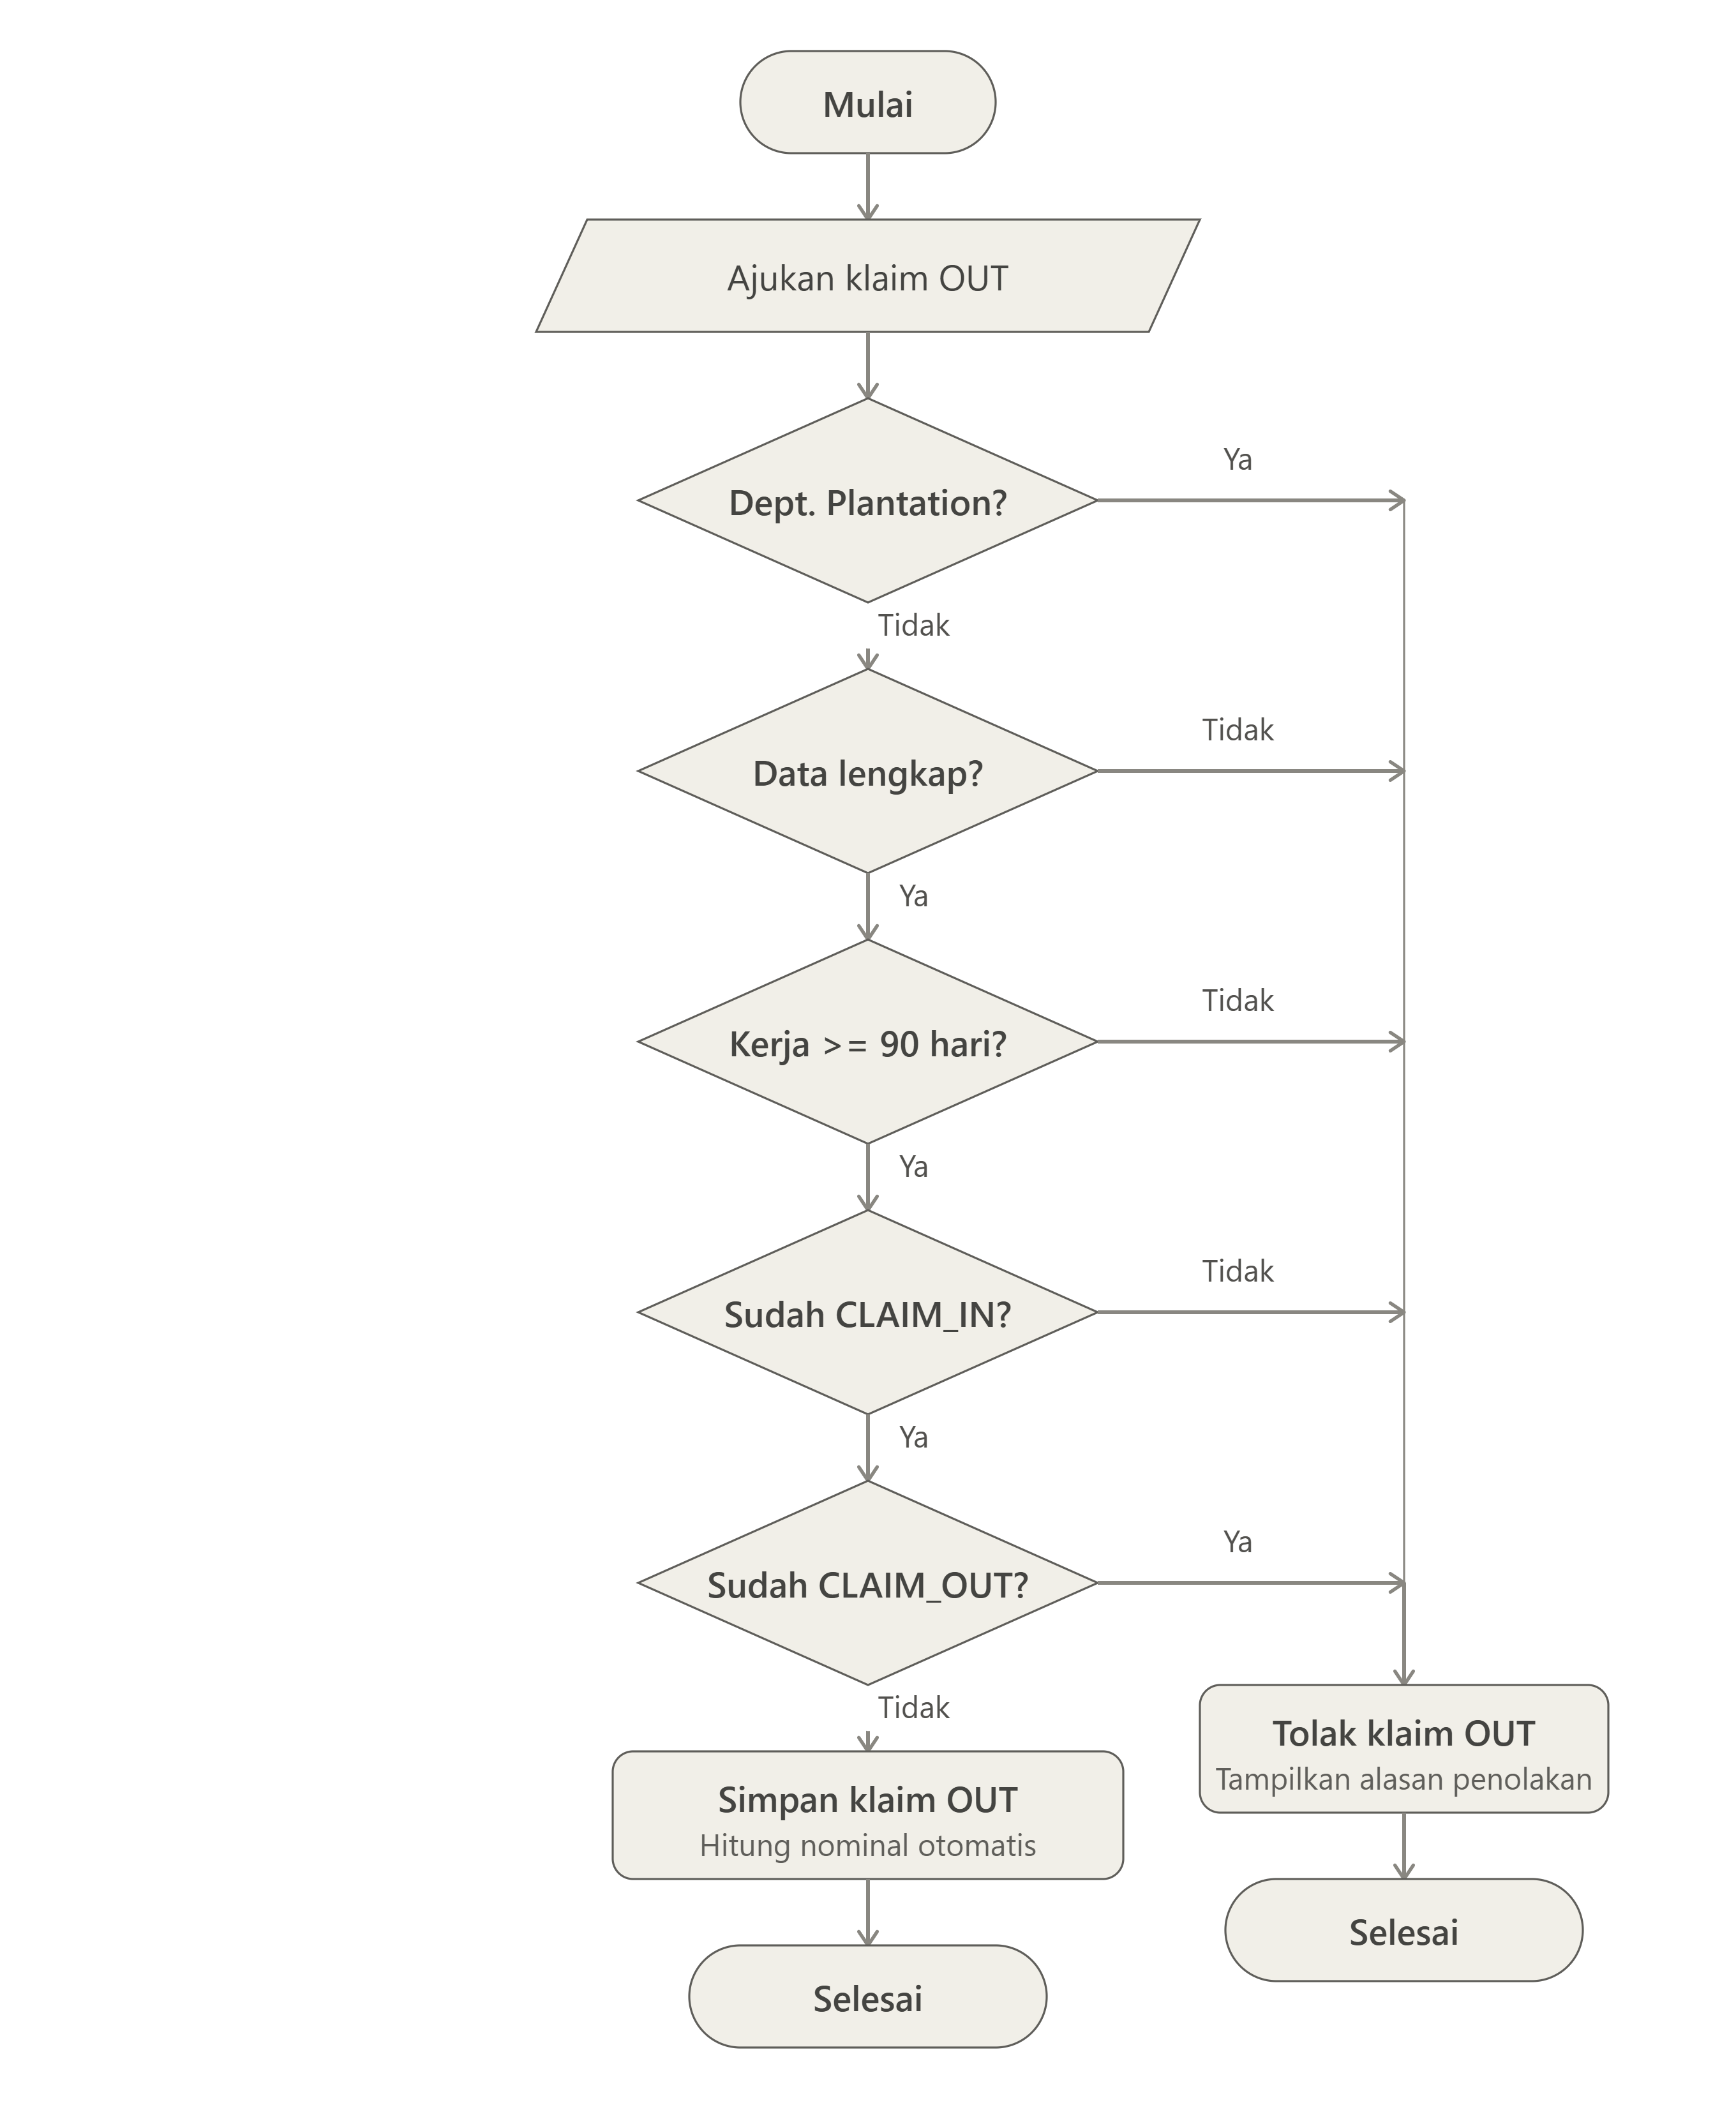
\includegraphics[width=0.85\textwidth]{assets/pics/flowchart_claim_out.png}
\caption{Flowchart validasi pengajuan Klaim Transport (CLAIM\_OUT)}
\label{fig:flowchart-claimout}
\end{figure}

\subsubsection*{Flowchart Surat Izin Keluar}

Rancangan alur pembentukan nomor referensi surat jalan otomatis serta pembaruan status karyawan sebagaimana diimplementasikan pada Kode \ref{lst:permit} ditunjukkan pada Gambar \ref{fig:flowchart-permit}.

\begin{figure}[H]
\centering
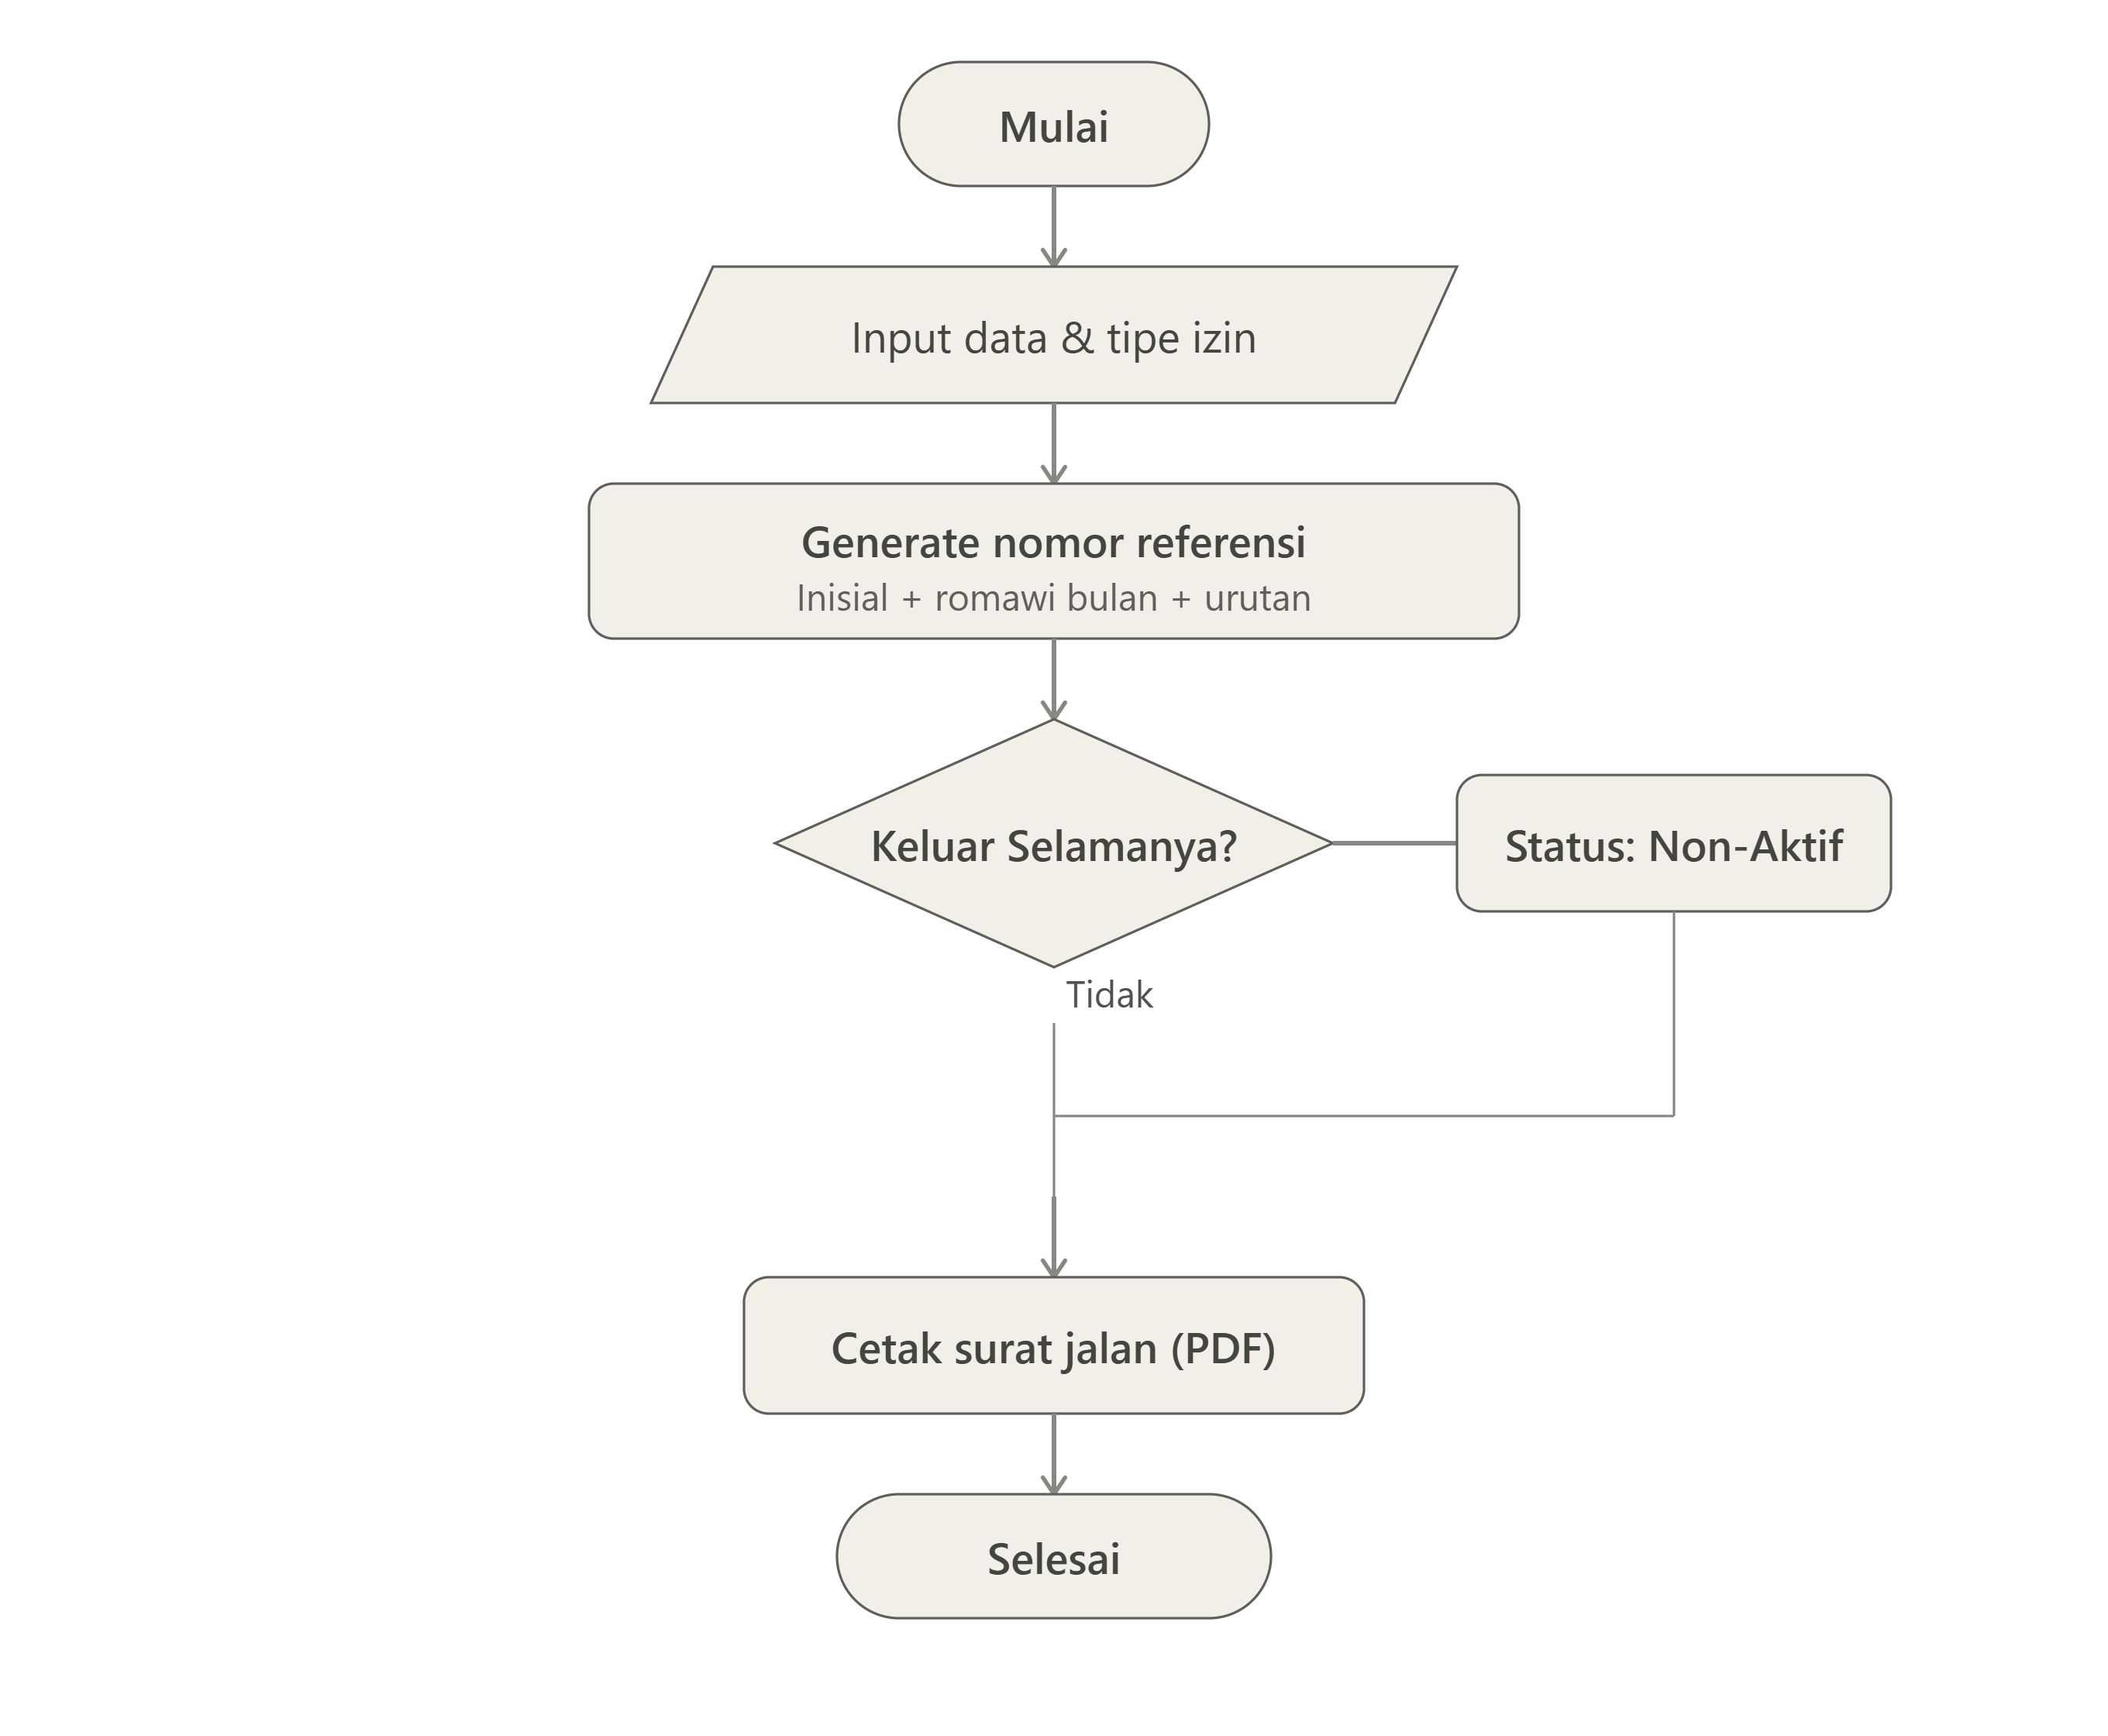
\includegraphics[width=0.8\textwidth]{assets/pics/flowchart_permit.png}
\caption{Flowchart proses Surat Izin Keluar}
\label{fig:flowchart-permit}
\end{figure}

\subsubsection*{Flowchart Manajemen Tarif Transport}

Rancangan alur pembaruan tarif transport secara atomik beserta mekanisme pengarsipan sebagaimana diimplementasikan pada Kode \ref{lst:rates} ditunjukkan pada Gambar \ref{fig:flowchart-rates}.

\begin{figure}[H]
\centering
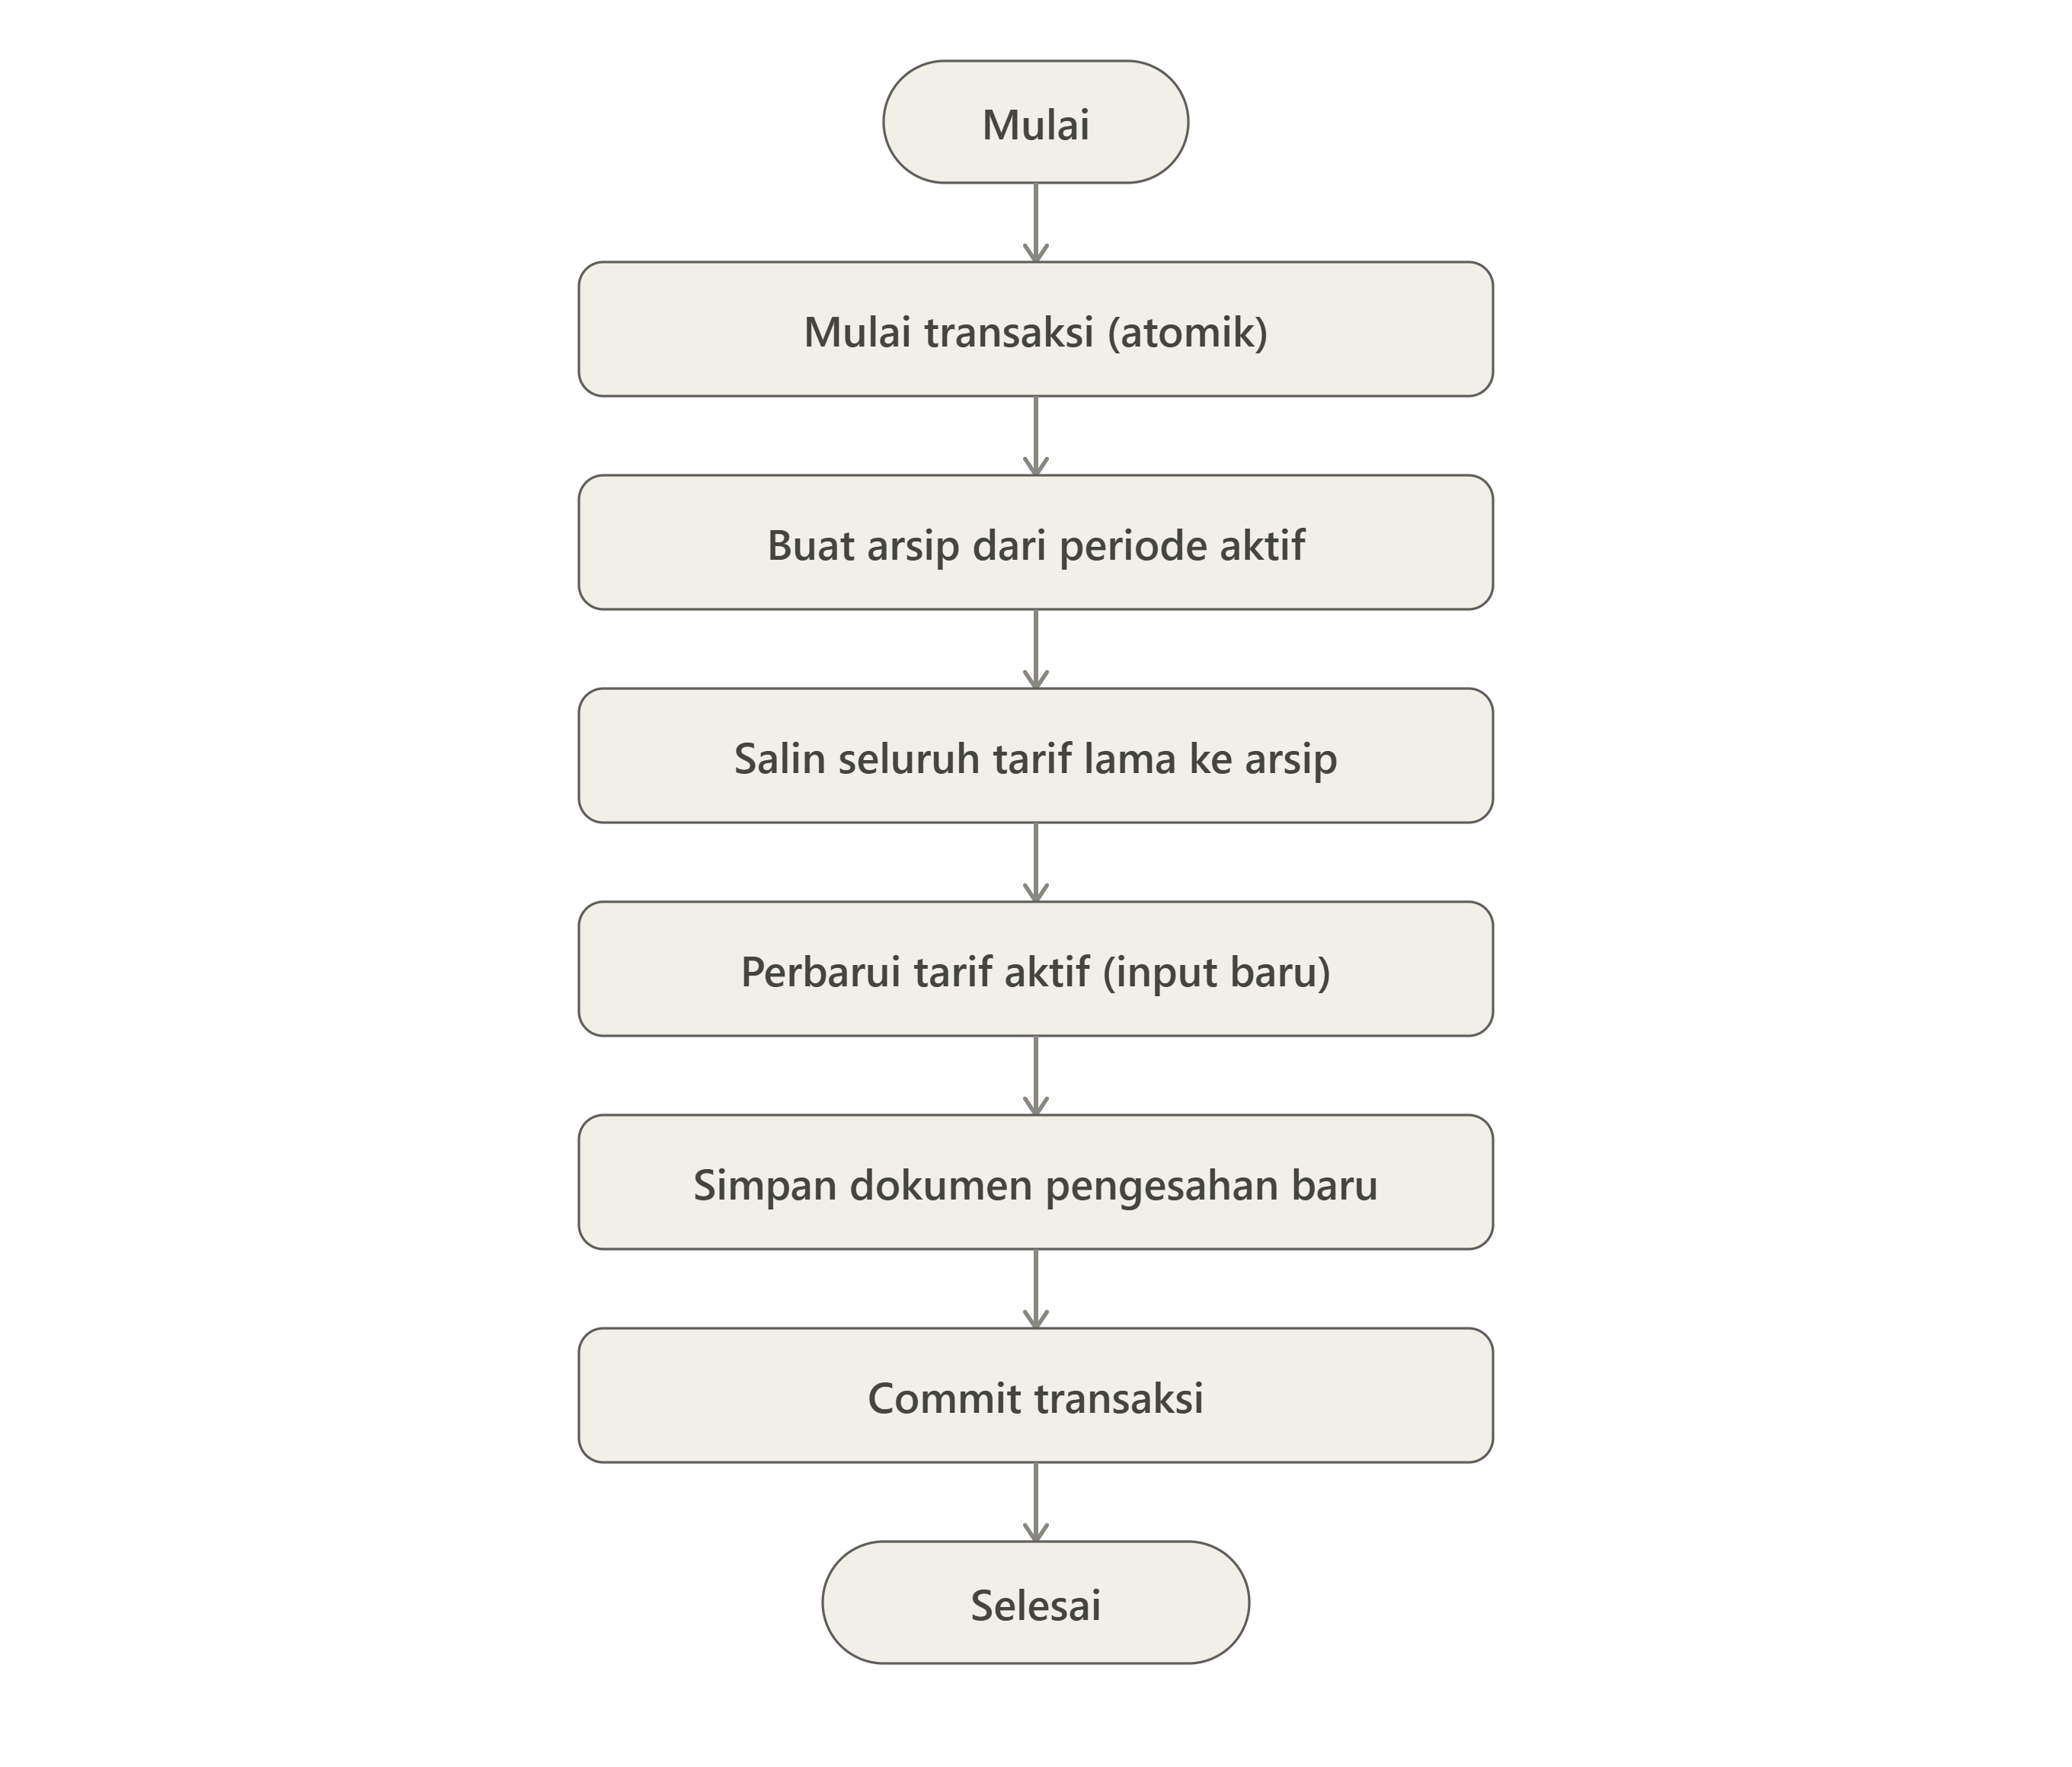
\includegraphics[width=0.8\textwidth]{assets/pics/flowchart_rates.png}
\caption{Flowchart proses Manajemen Tarif Transport}
\label{fig:flowchart-rates}
\end{figure}

\subsubsection*{Flowchart Persetujuan Karyawan}

Rancangan alur evaluasi kelengkapan data sebelum karyawan diaktifkan sebagaimana diimplementasikan pada Kode \ref{lst:approval} ditunjukkan pada Gambar \ref{fig:flowchart-approval}.

\begin{figure}[H]
\centering
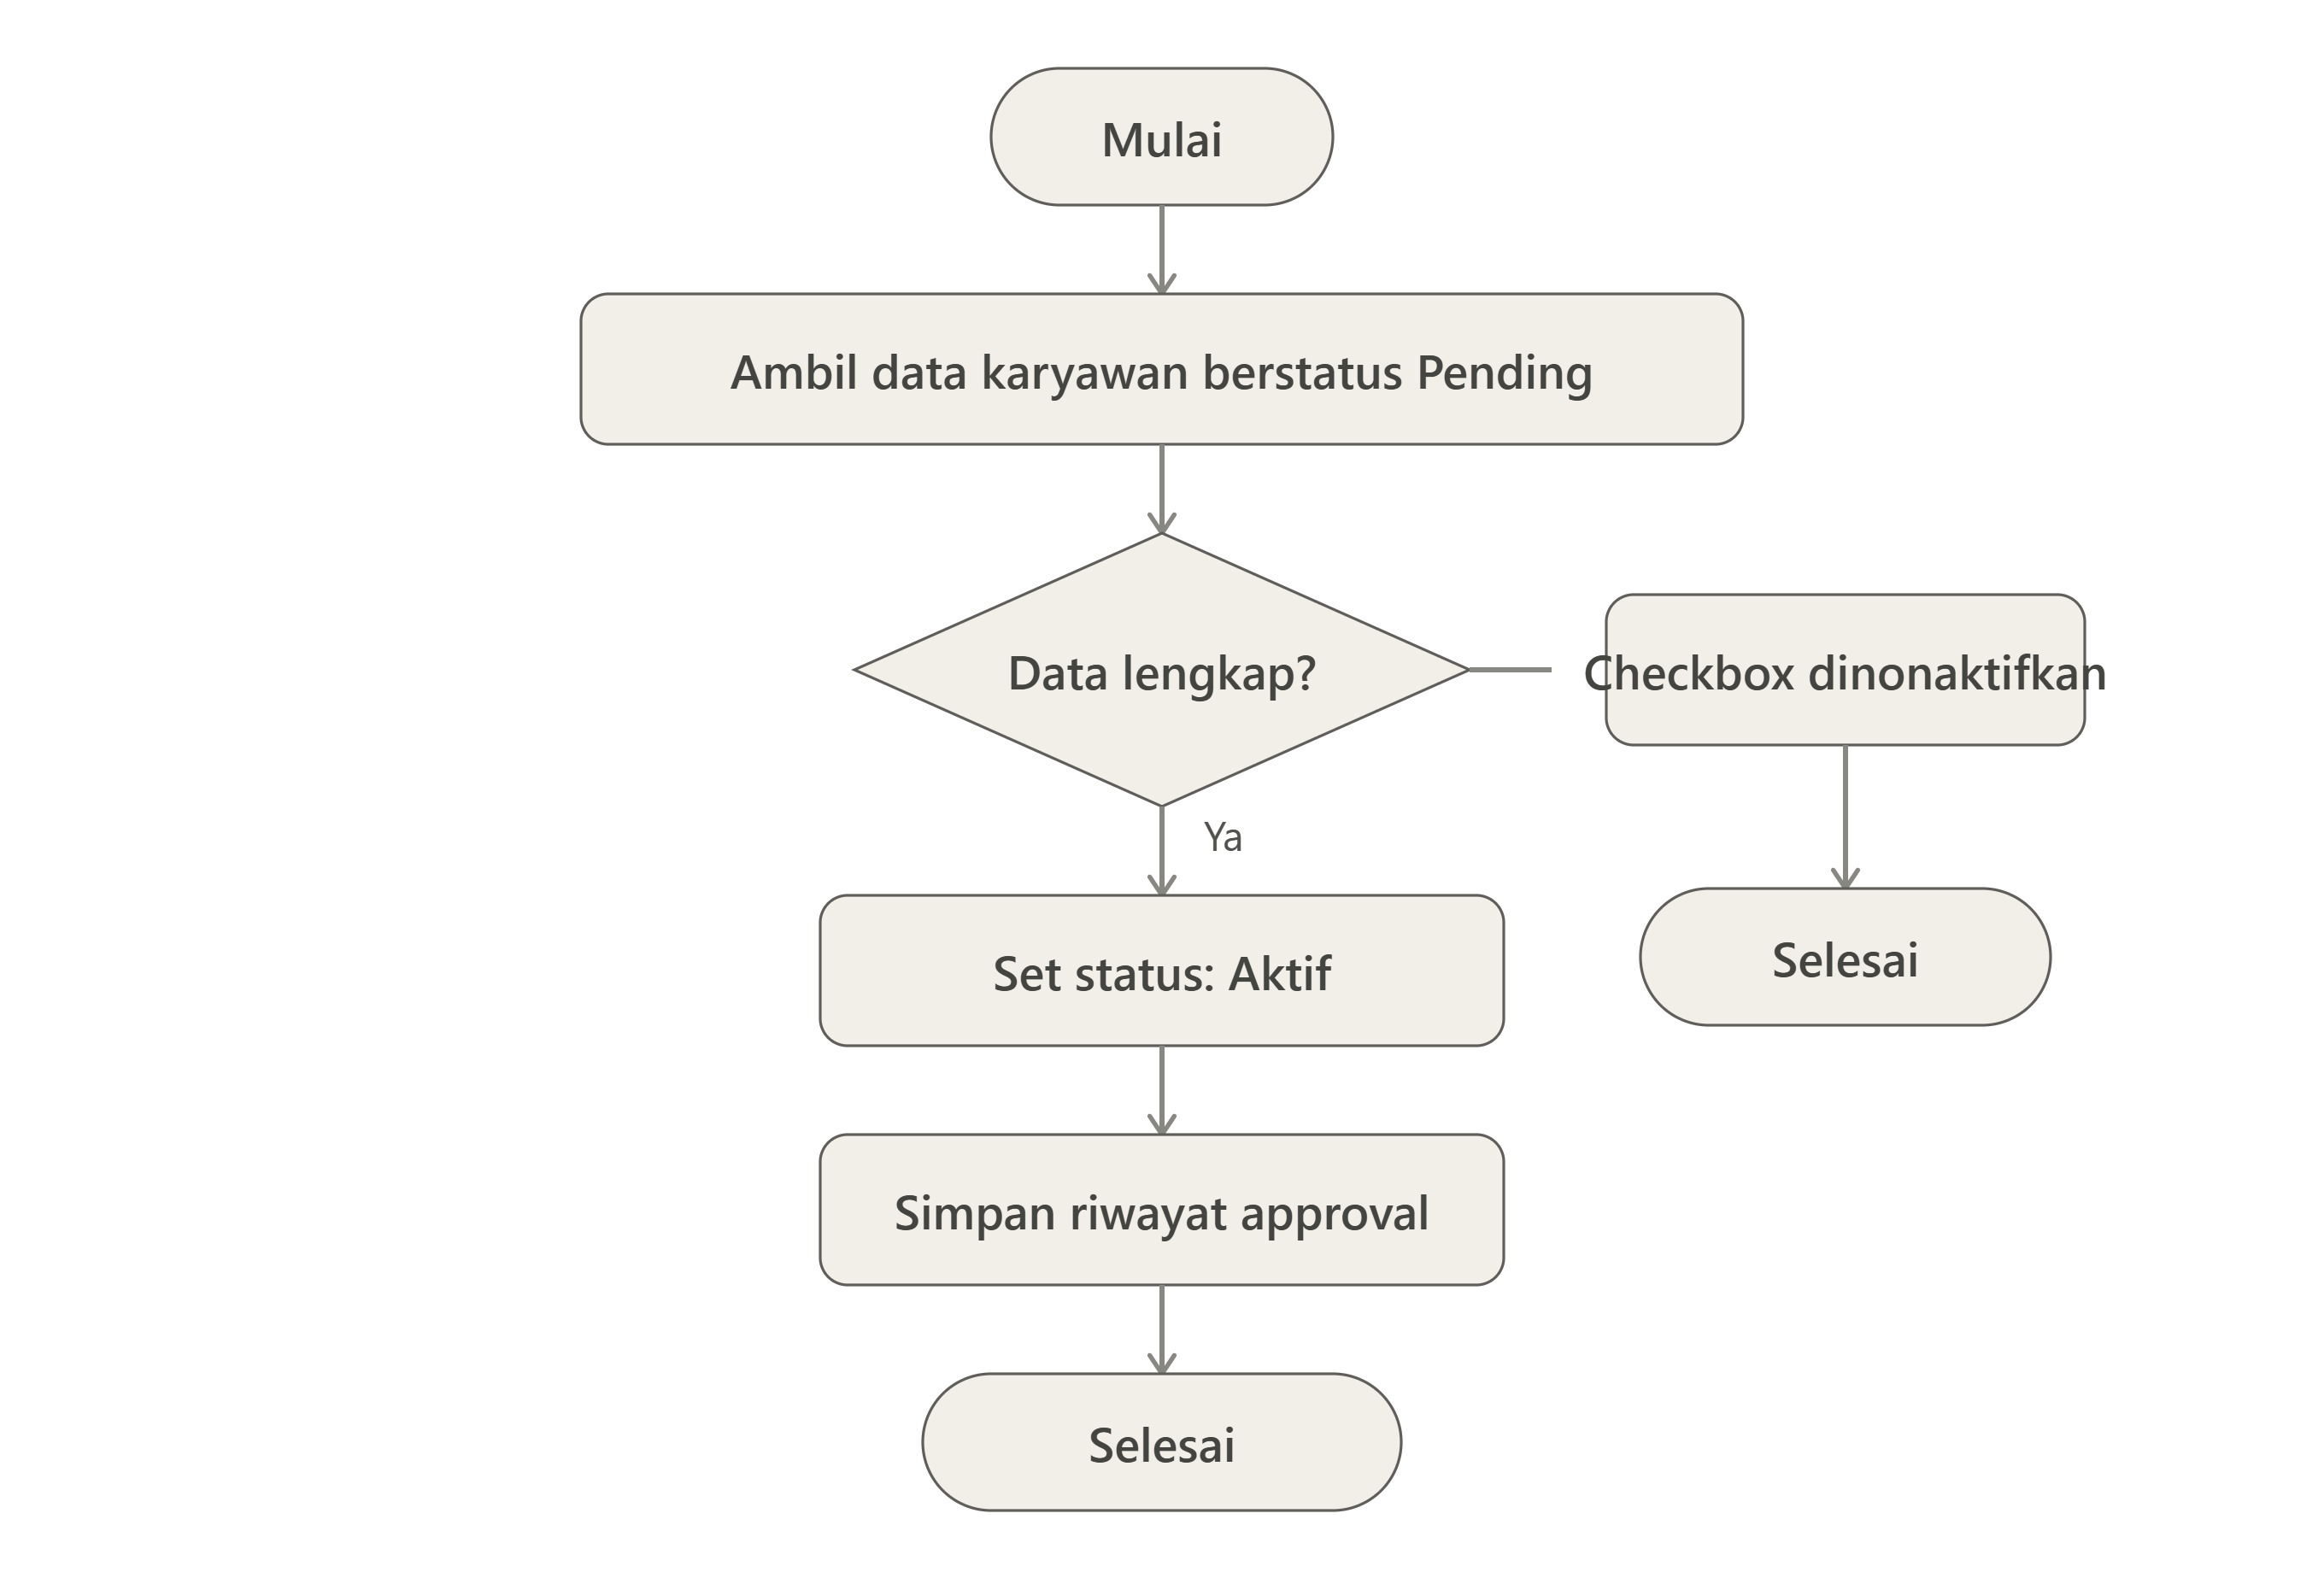
\includegraphics[width=0.8\textwidth]{assets/pics/flowchart_approval.png}
\caption{Flowchart proses Persetujuan Karyawan}
\label{fig:flowchart-approval}
\end{figure}

\subsubsection*{Flowchart RBAC (Manajemen Pengguna)}

Rancangan alur pembatasan akses menu berbasis peran sebagaimana diimplementasikan pada Kode \ref{lst:rbac} ditunjukkan pada Gambar \ref{fig:flowchart-rbac}.

\begin{figure}[H]
\centering
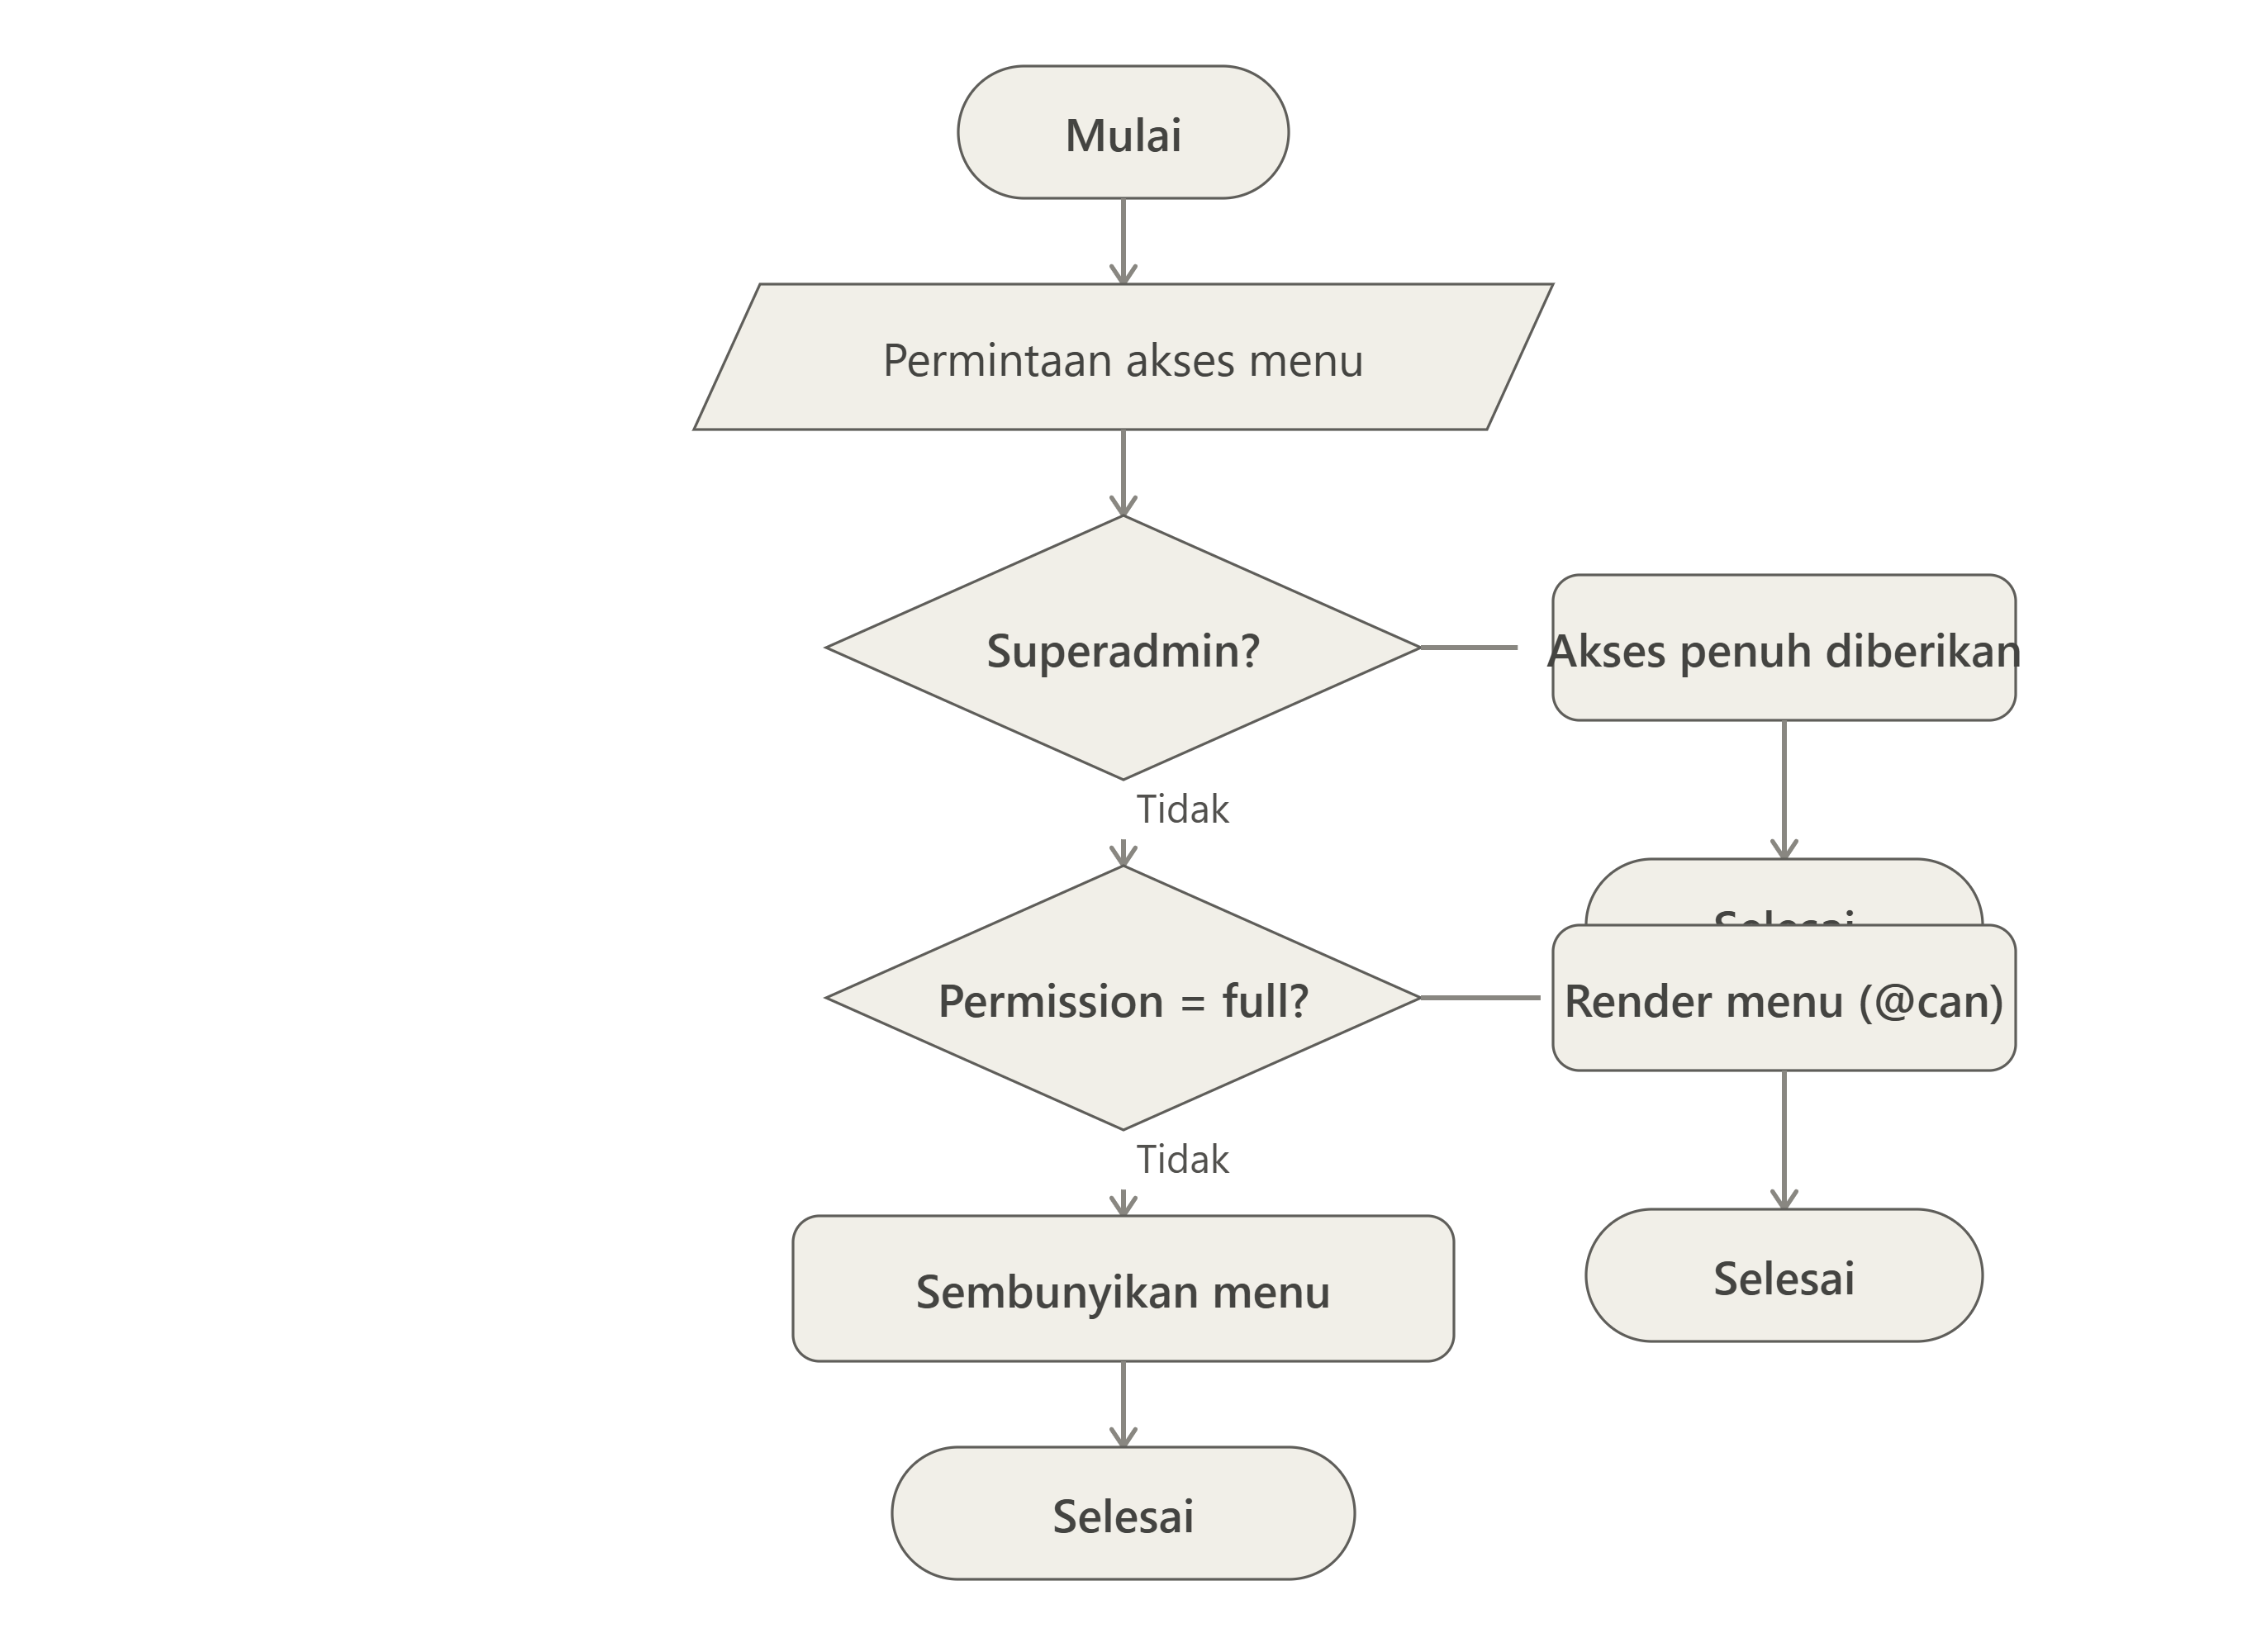
\includegraphics[width=0.8\textwidth]{assets/pics/flowchart_rbac.png}
\caption{Flowchart RBAC pada fitur Manajemen Pengguna}
\label{fig:flowchart-rbac}
\end{figure}

%-----------------------------------------------------------------------------%
\subsection{Implementasi Sistem}
%-----------------------------------------------------------------------------%
Selama pelaksanaan kerja magang, terdapat enam fitur utama yang dikembangkan dalam sistem \textit{HR Safety Campus} berdasarkan rancangan pada sub-bab sebelumnya. Berikut adalah uraian dari masing-masing fitur tersebut beserta cuplikan kode program inti yang merepresentasikan logika utamanya.

\subsubsection*{Registrasi Tenaga Kerja (\textit{Employee Registration})}

Fitur registrasi tenaga kerja merupakan pondasi utama dari seluruh sistem ini. Melalui fitur ini, staf HR dapat mendaftarkan tenaga kerja baru secara digital dengan mengisi data lengkap, mulai dari informasi pribadi seperti nama lengkap, NIK, tanggal lahir, dan jenis kelamin, hingga data kepegawaian seperti tanggal masuk kerja, jabatan, departemen, lokasi kantor, kontraktor yang menaungi, serta foto wajah tenaga kerja. Sistem juga dilengkapi penomoran ID karyawan otomatis dengan format tahun diikuti empat digit urutan (contoh: 20250001), pencarian wilayah bertingkat menggunakan data IndoRegion, penentuan status karyawan secara otomatis, fitur \textit{Re-Hire} untuk memulihkan data karyawan lama, serta cetak ID Card terintegrasi dalam format PDF menggunakan \textit{library} FPDF, sebagaimana telah dirancang pada Gambar \ref{fig:flowchart-registrasi}. Cuplikan logika pembuatan ID karyawan otomatis ditunjukkan pada Kode \ref{lst:reg}.

\begin{lstlisting}[language=PHP, caption={Logika pembuatan ID karyawan otomatis dan penentuan status pada fitur Registrasi}, label={lst:reg}]
// Membuat ID karyawan: tahun + 4 digit urutan (contoh: 20250001).
// Urutan diambil dari no_id terbesar tahun berjalan, bukan dari jumlah baris,
// agar tetap konsisten meskipun ada data yang dihapus.
$currentYear  = date('Y');
$lastEmployee = Employee::where('no_id', 'like', $currentYear . '%')
    ->orderBy('no_id', 'desc')
    ->first();

$newSequence = $lastEmployee
    ? ((int) substr($lastEmployee->no_id, 4)) + 1
    : 1;

$data['no_id'] = $currentYear . str_pad($newSequence, 4, '0', STR_PAD_LEFT);

// Status ditentukan otomatis: Aktif jika data lengkap, Pending jika belum.
$employee = new Employee($data);
$employee->status = $employee->isComplete() ? 'Aktif' : 'Pending';
$employee->save();
\end{lstlisting}

Kode \ref{lst:reg} mengilustrasikan mekanisme penomoran ID karyawan yang menjamin keunikan sekaligus konsistensi data, sesuai dengan rancangan alur pada Gambar \ref{fig:flowchart-registrasi}. Variabel \texttt{\$lastEmployee} mencari rekaman dengan \texttt{no\_id} terbesar pada tahun berjalan menggunakan \texttt{orderBy('no\_id', 'desc')}, bukan menghitung jumlah baris pada tabel --- pendekatan ini penting agar urutan penomoran tetap konsisten meskipun ada data yang dihapus di tengah proses. Selanjutnya, \texttt{str\_pad} memastikan format empat digit tetap terjaga (misalnya \texttt{0007}, bukan \texttt{7}). Pada bagian akhir, method \texttt{isComplete()} dipanggil untuk menentukan status awal karyawan secara otomatis, sehingga staf HR tidak perlu menetapkan status secara manual saat proses registrasi.

Antarmuka Main Menu yang menjadi pusat navigasi seluruh fitur sistem ditunjukkan pada Lampiran 9 Gambar A1, sementara halaman Manage Database Pegawai yang menampilkan daftar tenaga kerja beserta status pencetakan ID Card dapat dilihat pada Gambar A2. Formulir input data pribadi dan kepegawaian yang digunakan staf HR untuk mendaftarkan tenaga kerja baru ditunjukkan pada Gambar A3, memperlihatkan pembagian dua kolom data sesuai rancangan pada Kode \ref{lst:reg}.

\subsubsection*{Klaim Transport (\textit{Transport Claim})}

Fitur klaim transport dirancang untuk mengelola administrasi penggantian biaya transportasi bagi tenaga kerja kontrak yang berasal dari luar daerah. Sistem ini mengelola dua jenis klaim, yaitu \texttt{CLAIM\_IN} (klaim kedatangan) dan \texttt{CLAIM\_OUT} (klaim kepulangan), masing-masing dengan aturan bisnis yang ketat, sebagaimana telah dirancang pada Gambar \ref{fig:flowchart-claimin} dan Gambar \ref{fig:flowchart-claimout}. Untuk \texttt{CLAIM\_IN}, karyawan harus telah bekerja minimal 60 hari dan hanya diperbolehkan satu kali dalam setahun. Untuk \texttt{CLAIM\_OUT}, karyawan wajib sudah pernah melakukan \texttt{CLAIM\_IN} sebelumnya, dengan pengecualian karyawan dari departemen \textit{Plantation} yang tidak diperbolehkan mengajukan \texttt{CLAIM\_OUT}. Besaran nominal klaim dihitung otomatis berdasarkan kombinasi departemen dan provinsi asal karyawan, serta mendukung pemrosesan secara \textit{batch} untuk efisiensi waktu. Penerapan aturan bisnis berlapis seperti ini sejalan dengan temuan Zulkarnain dan Doke \cite{zulkarnain2026validasi}, yang menekankan bahwa validasi relasional yang ketat pada tingkat sistem berperan penting dalam menjaga integritas data transaksi sekaligus menutup celah inkonsistensi maupun kecurangan. Cuplikan validasi aturan klaim ditunjukkan pada Kode \ref{lst:claim}.

\begin{lstlisting}[language=PHP, caption={Validasi aturan bisnis berlapis pada fitur Klaim Transport}, label={lst:claim}]
$daysWorked  = Carbon::parse($emp->join_date)->diffInDays(now());
$hasClaimIn  = Claim::where('employee_id', $emp->id)->where('type', 'CLAIM_IN')->exists();
$hasClaimOut = Claim::where('employee_id', $emp->id)->where('type', 'CLAIM_OUT')->exists();

// Evaluasi syarat CLAIM_IN: minimal 60 hari kerja & maksimal 1x per tahun
$eligibleIn = true;
if (!$isComplete)            { $eligibleIn = false; $msgIn = 'Status/NIK/Finger kosong'; }
elseif ($daysWorked < 60)   { $eligibleIn = false; $msgIn = "Baru {$daysWorked} hari (min. 60)"; }
elseif ($hasClaimIn) {
    $last = Claim::where('employee_id', $emp->id)->where('type', 'CLAIM_IN')
        ->latest('date_claim')->first();
    if (Carbon::parse($last->date_claim)->diffInDays(now()) < 365)
        { $eligibleIn = false; $msgIn = 'Sudah CLAIM_IN dalam 1 tahun'; }
}

// Evaluasi syarat CLAIM_OUT: minimal 90 hari kerja & wajib sudah CLAIM_IN
$eligibleOut = true;
if (!$isComplete)           { $eligibleOut = false; }
elseif ($daysWorked < 90)   { $eligibleOut = false; $msgOut = "Baru {$daysWorked} hari (min. 90)"; }
elseif (!$hasClaimIn)       { $eligibleOut = false; $msgOut = 'Belum pernah CLAIM_IN'; }
elseif ($hasClaimOut)       { $eligibleOut = false; $msgOut = 'Sudah pernah CLAIM_OUT'; }

// Proteksi tambahan saat penyimpanan: departemen Plantation tidak boleh CLAIM_OUT
if ($request->type === 'CLAIM_OUT' && stripos($emp->department, 'Plantation') !== false) {
    continue; // lewati karyawan Plantation
}
\end{lstlisting}

Kode \ref{lst:claim} menunjukkan penerapan validasi berlapis yang dieksekusi secara berurutan menggunakan struktur \texttt{if-elseif}, sesuai dengan rancangan alur pada Gambar \ref{fig:flowchart-claimin} dan Gambar \ref{fig:flowchart-claimout}. Variabel \texttt{\$daysWorked} dihitung menggunakan \texttt{Carbon::diffInDays} untuk menentukan lama masa kerja karyawan terhitung sejak \texttt{join\_date}. Pada evaluasi \texttt{CLAIM\_IN}, sistem memeriksa riwayat klaim melalui \texttt{\$hasClaimIn}, kemudian membandingkan tanggal klaim terakhir (\texttt{\$last->date\_claim}) dengan tanggal saat ini untuk memastikan jeda minimal satu tahun. Sementara pada evaluasi \texttt{CLAIM\_OUT}, terdapat pengecualian khusus menggunakan \texttt{stripos(\$emp->department, 'Plantation')} yang secara otomatis melewati (\texttt{continue}) karyawan dari departemen \textit{Plantation}, sesuai kebijakan perusahaan yang tidak mengizinkan klaim kepulangan bagi departemen tersebut.

Lampiran 9 Gambar A4 menunjukkan antarmuka fitur \textit{Transport Claim}, memperlihatkan alur input rombongan berdasarkan vendor serta pemilihan jenis klaim (\texttt{CLAIM\_IN} atau \texttt{CLAIM\_OUT}) sebelum sistem melakukan validasi otomatis sesuai aturan bisnis pada Kode \ref{lst:claim}.

\subsubsection*{Surat Izin Keluar (\textit{Exit Permits})}

Fitur surat izin keluar mengelola proses administrasi ketika tenaga kerja akan meninggalkan area kerja, baik sementara (Keluar Kembali) maupun permanen (Keluar Selamanya), sebagaimana telah dirancang pada Gambar \ref{fig:flowchart-permit}. Setiap surat jalan yang diterbitkan mendapatkan nomor referensi unik yang digenerate secara otomatis dengan format yang mencakup inisial kontraktor, kode \textit{``PERMIT''}, angka romawi bulan, dan tahun (contoh: 0001/MMJ/PERMIT/VI/2025). Jika jenis izin yang dipilih adalah ``Keluar Selamanya'', sistem secara otomatis mengubah status karyawan menjadi Non-Aktif di basis data. Hasil akhirnya berupa surat jalan yang dapat dicetak dalam format A4 \textit{landscape}, lengkap dengan kop surat, tabel data karyawan, dan kolom tanda tangan. Cuplikan pembuatan nomor surat jalan otomatis ditunjukkan pada Kode \ref{lst:permit}.

\begin{lstlisting}[language=PHP, caption={Pembuatan nomor referensi surat jalan otomatis}, label={lst:permit}]
// Format: urutan/inisial-kontraktor/PERMIT/bulan-romawi/tahun
$initial = $this->getInitials($request->contractor_name); // "PT Maju Jaya" -> "MJ"
$romawi  = $this->getRomawi(now()->month);                // contoh: VI
$year    = now()->year;

$lastPermit = Permit::whereYear('created_at', $year)
    ->where('letter_reference', 'LIKE', "%/$initial/PERMIT/$romawi/$year")
    ->orderBy('id', 'desc')->first();

$newNumber = $lastPermit
    ? intval(explode('/', $lastPermit->letter_reference)[0]) + 1
    : 1;

$letterReference = sprintf('%04d/%s/PERMIT/%s/%s', $newNumber, $initial, $romawi, $year);

// Jika izin "Keluar Selamanya", status karyawan otomatis menjadi Non-Aktif
if ($request->type == 'Keluar Selamanya') {
    $employee->update(['status' => 'Non-Aktif']);
}
\end{lstlisting}

Kode \ref{lst:permit} menunjukkan pembentukan nomor referensi surat jalan yang unik dan terurut per kontraktor, sesuai rancangan pada Gambar \ref{fig:flowchart-permit}. Fungsi \texttt{getInitials} mengekstrak inisial dari nama kontraktor (misalnya ``PT Maju Jaya'' menjadi ``MJ''), sedangkan \texttt{getRomawi} mengonversi bulan berjalan ke format angka romawi sesuai konvensi penomoran surat resmi. Pencarian \texttt{\$lastPermit} menggunakan pola \texttt{LIKE} yang menyaring berdasarkan kombinasi inisial, bulan romawi, dan tahun yang sama, sehingga nomor urut hanya bertambah relatif terhadap kontraktor dan periode yang identik. Pada bagian akhir, kondisi \texttt{Keluar Selamanya} langsung memicu perubahan status karyawan menjadi \textit{Non-Aktif}, menghindari kebutuhan pembaruan status secara manual oleh staf HR.

Antarmuka fitur \textit{Exit Permits} yang menampilkan proses input rombongan, pemilihan tipe izin, serta pencetakan surat jalan ditunjukkan pada Lampiran 9 Gambar A5, sesuai dengan logika pembuatan nomor referensi otomatis pada Kode \ref{lst:permit}.

\subsubsection*{Manajemen Tarif Transport (\textit{Manage Rates})}

Fitur ini berfungsi sebagai acuan perhitungan klaim transportasi, sebagaimana telah dirancang pada Gambar \ref{fig:flowchart-rates}. HR Manager dapat mengelola master data tarif yang diorganisir berdasarkan dua dimensi utama, yaitu departemen (\textit{Harvesting} atau \textit{Plantation}) dan wilayah asal karyawan (provinsi). Setiap kombinasi memiliki tarif kedatangan (IN) dan kepulangan (OUT) yang berbeda-beda. Mekanisme pembaruan tarif dilengkapi sistem pengarsipan otomatis sehingga data lama tersimpan sebagai arsip untuk keperluan audit. Fitur ini juga mendukung pengunggahan dokumen PDF berupa surat pengesahan tarif resmi dari manajemen sebagai bukti legal penetapan tarif. Cuplikan mekanisme pengarsipan tarif lama ditunjukkan pada Kode \ref{lst:rates}.

\begin{lstlisting}[language=PHP, caption={Mekanisme pengarsipan otomatis saat pembaruan tarif}, label={lst:rates}]
DB::transaction(function () use ($data, $activePeriod, $newDocumentPath) {
    // 1. Buat periode arsip baru dari data periode aktif (untuk audit)
    $archive = RatePeriod::create([
        'name'          => 'Arsip per ' . Carbon::now()->format('d M Y H:i'),
        'start_date'    => $activePeriod->start_date,
        'end_date'      => Carbon::now(),
        'is_active'     => false,
        'document_path' => $activePeriod->document_path,
    ]);

    // 2. Salin seluruh tarif lama ke periode arsip
    foreach ($activePeriod->rates as $old) {
        TransportRate::create([
            'period_id'  => $archive->id,
            'department' => $old->department,
            'origin'     => $old->origin,
            'amount_in'  => $old->amount_in,
            'amount_out' => $old->amount_out,
        ]);
    }

    // 3. Perbarui tarif pada periode aktif dengan input baru
    foreach ($data['rates'] as $id => $val) {
        TransportRate::where('id', $id)->update([
            'amount_in'  => $val['amount_in'],
            'amount_out' => $val['amount_out'],
        ]);
    }

    $activePeriod->document_path = $newDocumentPath; // surat pengesahan PDF baru
    $activePeriod->save();
});
\end{lstlisting}

Kode \ref{lst:rates} memperlihatkan penggunaan \texttt{DB::transaction} untuk membungkus tiga langkah pembaruan tarif secara atomik, sesuai rancangan pada Gambar \ref{fig:flowchart-rates} --- artinya seluruh langkah akan dibatalkan (\textit{rollback}) apabila salah satu proses gagal, sehingga data tarif tidak pernah berada dalam kondisi tidak konsisten. Langkah pertama membuat rekaman arsip baru dari data periode aktif saat ini, diikuti penyalinan seluruh tarif lama ke dalam arsip tersebut pada langkah kedua. Barulah pada langkah ketiga, nilai tarif pada periode aktif diperbarui sesuai input baru. Pola ``arsipkan dahulu sebelum memperbarui'' ini memastikan jejak audit tarif lama tetap tersimpan dan dapat ditelusuri kembali kapan pun diperlukan.

Lampiran 9 Gambar A6 menunjukkan antarmuka \textit{Manage Rates}, menampilkan tabel tarif aktif berdasarkan kombinasi departemen dan provinsi asal karyawan, sekaligus fitur unggah dokumen pengesahan tarif sebagaimana dijelaskan pada Kode \ref{lst:rates}.

\subsubsection*{Persetujuan Karyawan (\textit{Employees Approval})}

Fitur \textit{approval} merupakan lapisan kontrol kualitas data sebelum seorang tenaga kerja resmi dianggap aktif dalam sistem, sebagaimana telah dirancang pada Gambar \ref{fig:flowchart-approval}. Karyawan yang didaftarkan dengan data belum lengkap akan berstatus \textit{Pending} dan muncul di halaman ini. Sistem secara otomatis mengevaluasi kelengkapan data dan menampilkan label ``Data Lengkap (Siap \textit{Approve})'' atau ``Data Belum Lengkap'' pada setiap baris. Karyawan dengan data tidak lengkap tidak dapat dipilih untuk di-\textit{approve} karena \textit{checkbox}-nya dinonaktifkan otomatis. Admin dapat melakukan \textit{approval} secara massal, dan setiap perubahan status tercatat dalam riwayat histori karyawan untuk keperluan \textit{audit trail}. Cuplikan evaluasi kelengkapan data ditunjukkan pada Kode \ref{lst:approval}.

\begin{lstlisting}[language=PHP, caption={Evaluasi kelengkapan data sebelum proses persetujuan}, label={lst:approval}]
// Memeriksa kelengkapan seluruh field wajib sebelum karyawan dapat di-approve.
// Jika salah satu field kosong, checkbox approval pada antarmuka dinonaktifkan.
public function isComplete()
{
    $required = [
        'no_id', 'fingerprint_id', 'nik', 'birth_date', 'gender',
        'address', 'province', 'regency', 'district', 'pic',
        'department', 'office_location', 'join_date', 'position',
        'contractor_id', 'group_leader', 'photo_path',
    ];

    foreach ($required as $field) {
        if (empty($this->$field)) {
            return false; // data belum lengkap
        }
    }
    return true;
}

// Saat proses approval massal, sistem memvalidasi ulang sebelum mengaktifkan
if ($emp && $emp->isComplete()) {
    $emp->status = 'Aktif';
    $emp->save();
}
\end{lstlisting}

Kode \ref{lst:approval} menunjukkan method \texttt{isComplete()} yang memeriksa 17 \textit{field} wajib secara \textit{looping}, dan langsung mengembalikan nilai \texttt{false} pada iterasi pertama begitu ditemukan \textit{field} yang kosong, sesuai rancangan pada Gambar \ref{fig:flowchart-approval}. Method ini dipanggil di dua titik berbeda: pada antarmuka untuk menonaktifkan \textit{checkbox} persetujuan, dan pada proses \textit{backend} saat \textit{approval} massal dieksekusi. Validasi ganda pada sisi \textit{backend} ini penting sebagai lapisan keamanan tambahan, karena mencegah karyawan dengan data tidak lengkap berstatus \textit{Aktif} meskipun ada upaya manipulasi permintaan (\textit{request}) dari sisi klien.

Antarmuka fitur \textit{Employees Approval} yang menampilkan daftar karyawan berstatus \textit{Pending} beserta label kelengkapan data ditunjukkan pada Lampiran 9 Gambar A7, merepresentasikan mekanisme evaluasi otomatis pada Kode \ref{lst:approval}.

\subsubsection*{Manajemen Pengguna (\textit{User Management})}

Fitur ini memberikan kemampuan kepada administrator sistem untuk mengelola hak akses pengguna aplikasi, sebagaimana telah dirancang pada Gambar \ref{fig:flowchart-rbac}. Administrator dapat membuat akun pengguna baru, mengatur \textit{password} awal, dan menentukan hak akses secara granular per menu, meliputi akses ke menu Registrasi, \textit{Permit Letter}, \textit{Transport Claim}, dan \textit{Manage Rates}. Sistem mengenal dua level pengguna, yaitu Administrator yang memiliki akses penuh ke seluruh fitur, dan \textit{User} biasa yang hanya dapat mengakses menu yang secara eksplisit diizinkan. Penerapan pembatasan akses ini mengadopsi konsep \textit{Role-Based Access Control} (RBAC) sebagaimana dijelaskan oleh Mary dan Febriyani \cite{mary2025rbac}. Pada sistem ini, RBAC diimplementasikan menggunakan mekanisme \textit{Gate} bawaan Laravel yang didefinisikan secara terpusat. Pengguna dengan atribut \textit{administrator} memperoleh akses penuh melalui \texttt{Gate::before}, sedangkan pengguna biasa hanya dapat membuka menu yang secara eksplisit diizinkan pada kolom \textit{permissions}, sesuai prinsip \textit{least privilege}. Setiap akun memiliki status yang dapat dikontrol: \textit{Active}, \textit{Pending}, atau \textit{Inactive}, serta terdapat mekanisme keamanan yang mencegah administrator menghapus akun miliknya sendiri secara tidak sengaja. Cuplikan definisi \textit{Gate} RBAC ditunjukkan pada Kode \ref{lst:rbac}.

\begin{lstlisting}[language=PHP, caption={Definisi Gate RBAC untuk pembatasan akses menu berdasarkan peran}, label={lst:rbac}]
// Super admin: akses penuh ke seluruh menu sebelum gerbang lain dievaluasi
Gate::before(function ($user, $ability) {
    if ($user->email === 'adminhrsc@gmail.com' || $user->is_admin) {
        return true;
    }
});

// Gerbang akses per menu (prinsip least privilege)
Gate::define('access-registration', fn ($user) =>
    ($user->permissions['registration'] ?? '') === 'full');

Gate::define('access-permit', fn ($user) =>
    ($user->permissions['permit'] ?? '') === 'full');

Gate::define('access-claim', fn ($user) =>
    ($user->permissions['claim'] ?? '') === 'full');

Gate::define('access-rates', fn ($user) =>
    ($user->permissions['rates'] ?? '') === 'full');

// Pada antarmuka Blade, menu hanya dirender bila pengguna berwenang:
// @can('access-claim') ... @endcan
\end{lstlisting}

Kode \ref{lst:rbac} menunjukkan penerapan RBAC menggunakan mekanisme \textit{Gate} bawaan Laravel, sesuai rancangan pada Gambar \ref{fig:flowchart-rbac}. Fungsi \texttt{Gate::before} dievaluasi terlebih dahulu sebelum \textit{gate} lainnya --- apabila pengguna cocok dengan kondisi \textit{superadmin} (email tertentu atau atribut \texttt{is\_admin}), akses penuh langsung diberikan tanpa perlu memeriksa \textit{gate} per menu. Setiap \texttt{Gate::define} merepresentasikan satu modul (misalnya \texttt{access-claim} yang berkorespondensi langsung dengan \textit{middleware} \texttt{can:access-claim} pada \textit{routing} sistem), yang memeriksa nilai pada kolom \texttt{permissions} milik pengguna. Pada sisi antarmuka, direktif Blade \texttt{@can} memastikan menu hanya dirender apabila pengguna berwenang, sehingga pembatasan akses diterapkan secara konsisten baik di sisi \textit{backend} maupun \textit{frontend}.

Halaman daftar pengguna beserta peran masing-masing ditunjukkan pada Lampiran 9 Gambar A8, sedangkan formulir penambahan pengguna baru beserta pengaturan hak akses granular per menu (RBAC) ditunjukkan pada Gambar A9, sesuai dengan definisi \textit{Gate} pada Kode \ref{lst:rbac}.

%-----------------------------------------------------------------------------%
\subsection{Kendala yang Ditemukan}
%-----------------------------------------------------------------------------%
Dalam proses pengembangan sistem \textit{HR Safety Campus}, terdapat beberapa kendala teknis dan operasional yang dihadapi selama pelaksanaan kerja magang, di antaranya:

\begin{enumerate}
    \item \textbf{Penyiapan Lingkungan Awal:} Pada tahap awal pengerjaan, sempat terjadi masalah kompatibilitas di perangkat pengembangan baru, di mana \textit{Composer} dan beberapa ekstensi PHP tidak terbaca oleh sistem.
    \item \textbf{Migrasi dan Duplikasi Data Masif:} Saat melakukan migrasi data dari sistem lama, ditemukan banyak sekali duplikasi data tenaga kerja (mencapai puluhan rekaman), terutama pada kolom NIK yang seharusnya unik. Hal ini membuat proses unggah (\textit{upload}) gagal karena melanggar aturan integritas basis data.
\end{enumerate}

%-----------------------------------------------------------------------------%
\subsection{Solusi atas Kendala yang Ditemukan}
%-----------------------------------------------------------------------------%
Solusi yang diterapkan untuk mengatasi kendala-kendala yang ditemukan selama proses pelaksanaan kerja magang adalah sebagai berikut:

\begin{enumerate}
    \item \textbf{Solusi Penyiapan Lingkungan Awal:} Masalah ini diselesaikan dengan melakukan \textit{troubleshooting} pada konfigurasi \textit{environment variables} di sistem operasi dan menginstal ulang paket yang dibutuhkan hingga server pengembangan lokal dapat berjalan dengan normal.
    \item \textbf{Solusi Migrasi dan Duplikasi Data Masif:} Skrip khusus dibuat untuk menyeleksi dan memisahkan data yang ganda melalui tiga lapis pemeriksaan, yaitu validasi format Nomor Induk Kependudukan (NIK) sebagai 16 digit angka murni, pengecekan duplikasi di dalam berkas unggahan yang sama, dan pengecekan duplikasi terhadap data yang sudah tersimpan pada basis data. Rekaman yang lolos seluruh pemeriksaan dikumpulkan sebagai data valid untuk diunggah, sementara rekaman bermasalah dicatat secara terpisah agar dapat dilaporkan kembali kepada klien, bukan dihapus begitu saja tanpa jejak. Sebelum melakukan pembersihan data dengan perintah \textit{TRUNCATE} dan mengunggah ulang \textit{file} CSV yang baru, konfirmasi temuan duplikat ini selalu dilakukan kepada pihak klien untuk memastikan tidak ada data pekerja sah yang tidak sengaja terhapus. Pendekatan deduplikasi berbasis seleksi ini sejalan dengan studi Ravikanth et al. \cite{ravikanth2024deduplication} mengenai pencocokan rekaman otomatis.
\end{enumerate}